\chapter{Resultados}
%\section{Resultados en Simulaci\'on}
\section {Resultados del Controlador Polar}
\begin{figure}[ht!]
     \begin{center}
        \subfigure[Evolución en la posición (x)]{\label{fig:etiquetaA}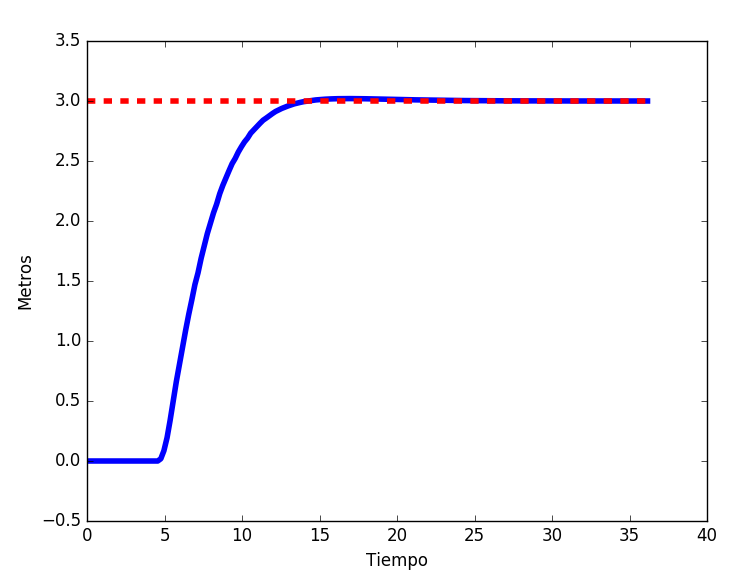
\includegraphics
        [width=.45\textwidth]{images/tvsxy_tesis.png}}
        \subfigure[Evolución de la velocidad lineal]{\label{fig:etiquetaB}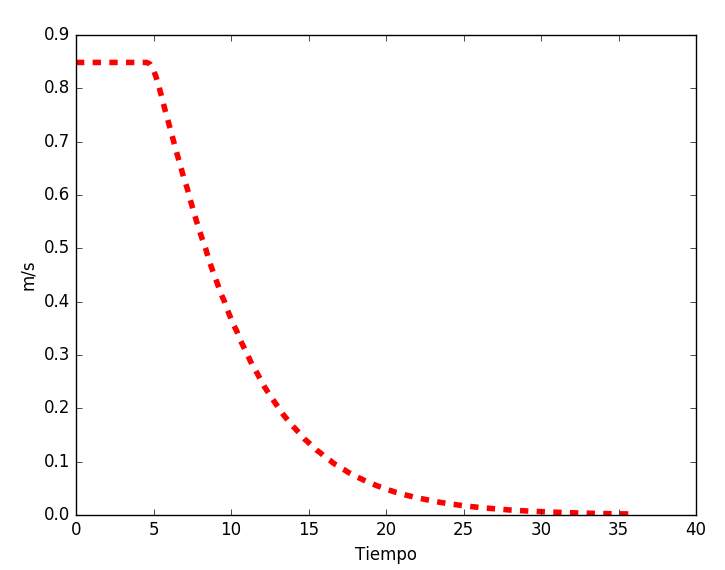
\includegraphics
        [width=.45\textwidth]{images/tvsv_tesis.png}}
        \subfigure[Evolución de la orientación]{\label{fig:etiquetaC}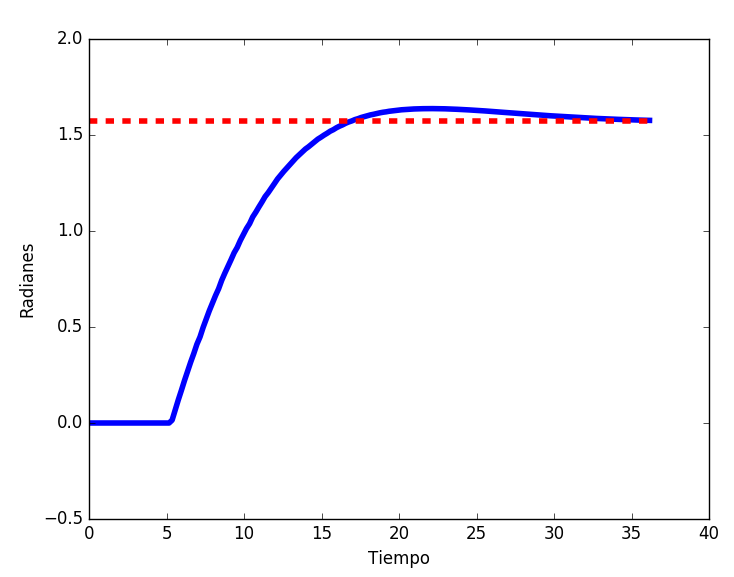
\includegraphics
        [width=.45\textwidth]{images/tvstheta_tesis.png}}
        \subfigure[Evolución de la velocidad angular]{\label{fig:etiquetaD}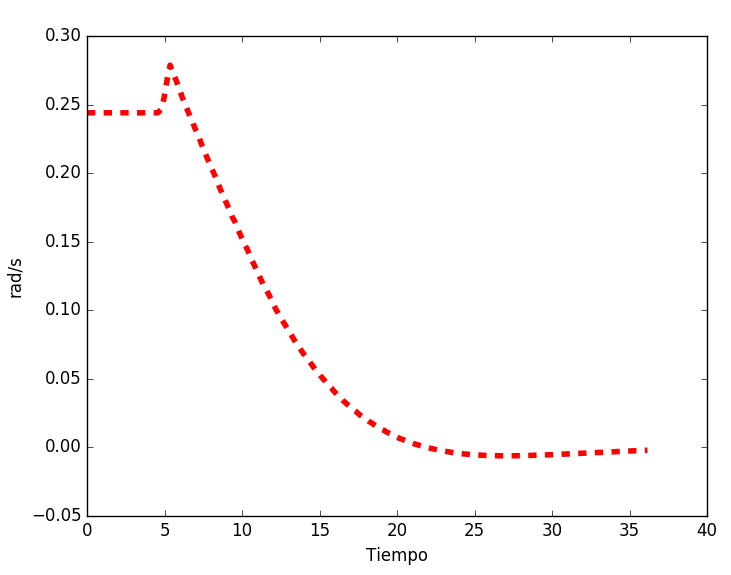
\includegraphics
        [width=.45\textwidth]{images/tvsomega_tesis.png}}
    \end{center}
  \captionsetup{font=footnotesize}
    \caption{\label{f:PolarControl}Evolución temporal de las variables de estado usando el controlador polar para lograr una posición deseada dada por $x = 3, y = 3, \theta = 90$}
\end{figure}

%\begin{figure}%[ht!]
%  \centering \footnotesize
%  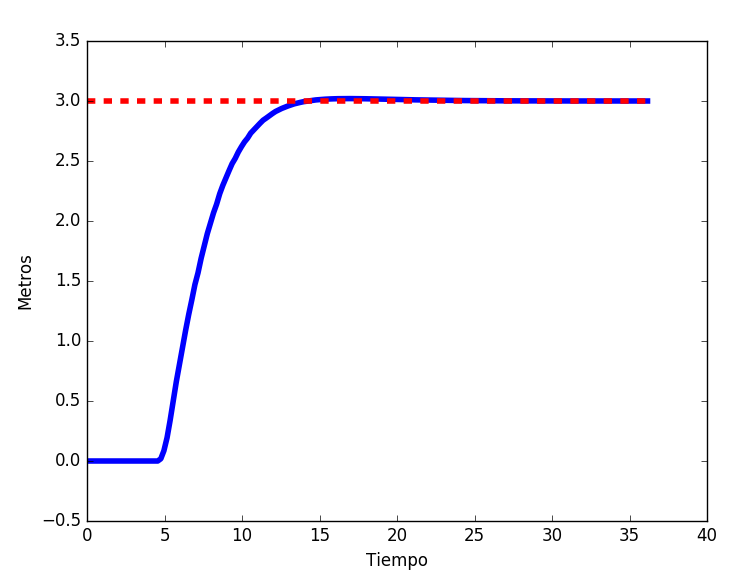
\includegraphics[width=0.49\textwidth]{images/tvsxy_tesis.png}
%  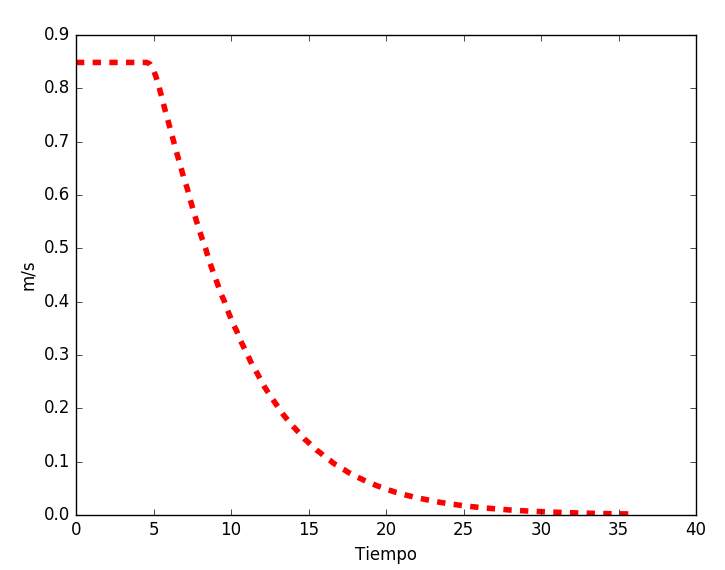
\includegraphics[width=0.49\textwidth]{images/tvsv_tesis.png}
%  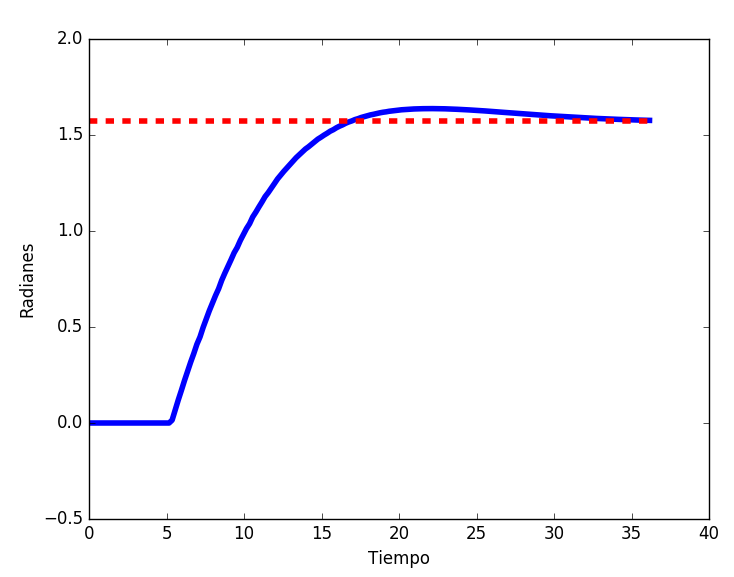
\includegraphics[width=0.49\textwidth]{images/tvstheta_tesis.png}
%  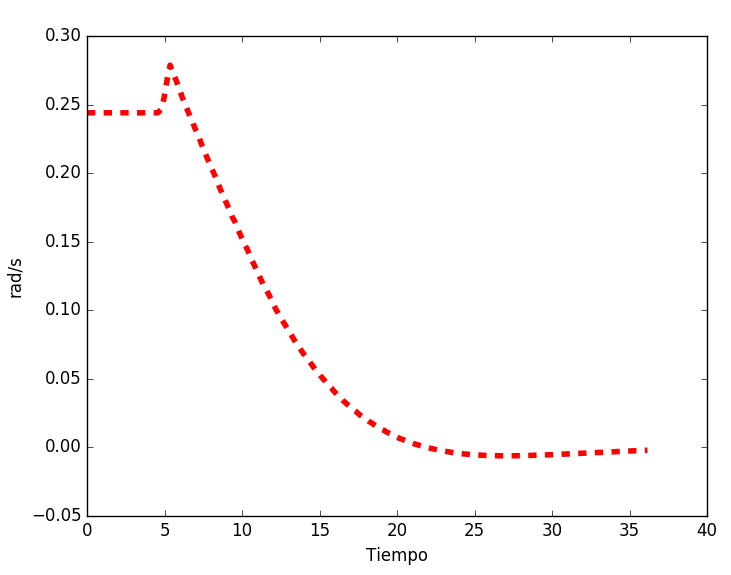
\includegraphics[width=0.49\textwidth]{images/tvsomega_tesis.png}
%  \captionsetup{font=footnotesize}
%  \caption{Evolución temporal de las variables de estado usando el controlador polar 
%  para lograr una posición deseada dada por $x = 3, y = 3, \theta = 90$}
%  \label{f:PolarControl}
%\end{figure}
Para probar el controlador polar, se usó una simulación dinámica en Gazebo con el robot 
Kobuki sin obstáculos, y las variables de estado que incluyen velocidad, posición y 
orientación se obtuvieron en línea a partir de la odometría simulada. Usando la información 
de esta odometría, el controlador se aplicó en línea. Para estas pruebas, la posición deseada
es $(x = 3, y = 3)$ y la orientación deseada $\theta = 90^{\circ}$. La figura 
\ref{f:PolarControl} (a) muestra la evolución temporal de la posición ($x$) donde 
se logra una convergencia a la posición deseada en menos de 20 segundos. Esto se debe a 
la distancia hacia el obstáculo. Diferentes distancias conducen a diferentes tiempos de 
convergencia, y la tasa de convergencia también se puede modificar cambiando las 
ganancias en \ref{eqn:w} para la velocidad angular, y en \ref{eqn:v} para la velocidad 
lineal. Las otras subfiguras en la figura \ref{f:PolarControl} muestran la evolución 
temporal de la velocidad lineal en $x$, la orientación y la velocidad angular. Para la 
orientación, hay un sobreimpulso que se debe a la excesiva dependencia del controlador 
en la posición en lugar de la orientación.
%\section{An\'alisis del mapa obtenido}
%\section{Resultados en un ambiente real}
\section{Resultados del Sistema de Navegación}
\begin{figure}[ht!]
     \begin{center}
        \subfigure[Fuerzas de atracción aplicado al robot móvil]{\label{fig:etiquetaA}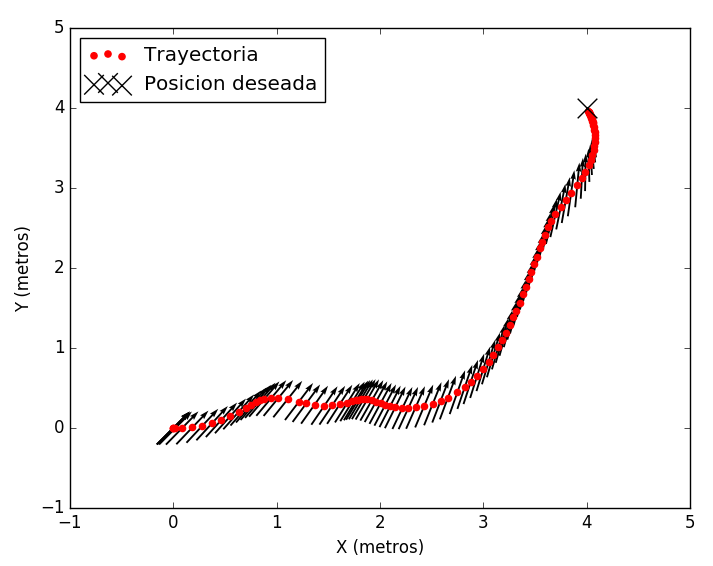
\includegraphics
        [width=.49\textwidth]{images/attr_kbki.png}}
        \subfigure[Fuerzas de repulsión aplicado al robot móvil]{\label{fig:etiquetaB}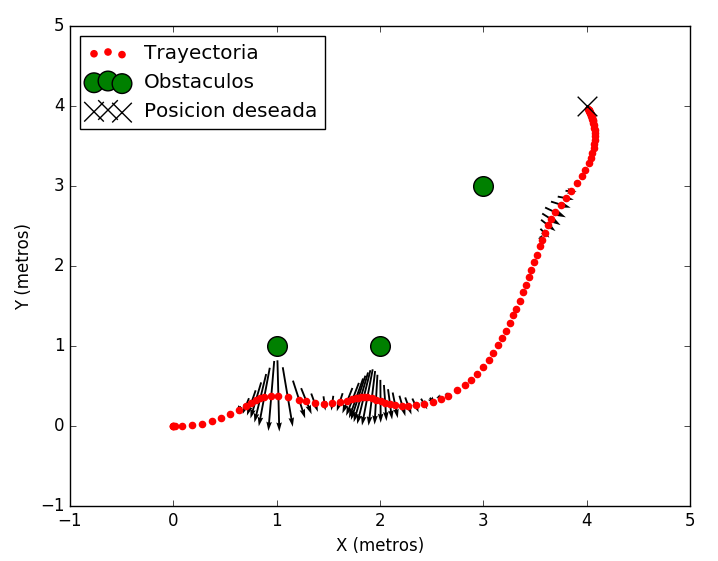
\includegraphics
        [width=.49\textwidth]{images/rep_kbki.png}}
        \subfigure[Fuerzas de navegación aplicado al robot móvil]{\label{fig:etiquetaC}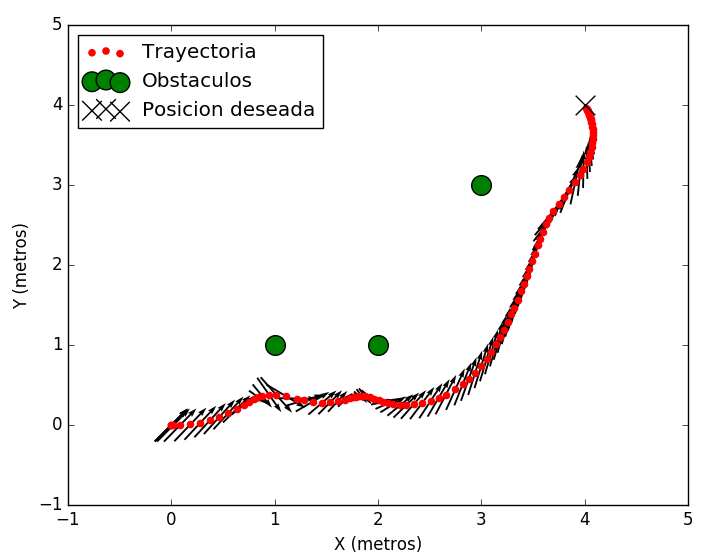
\includegraphics
        [width=.49\textwidth]{images/nav_kbki.png}}
    \end{center}
  \captionsetup{font=footnotesize}
    \caption{\label{f:kbki_APF}Navegación autónoma implementada en el robot diferencial Kobuki.}
\end{figure}

%\begin{figure}%[ht!]
%  \centering \footnotesize
%  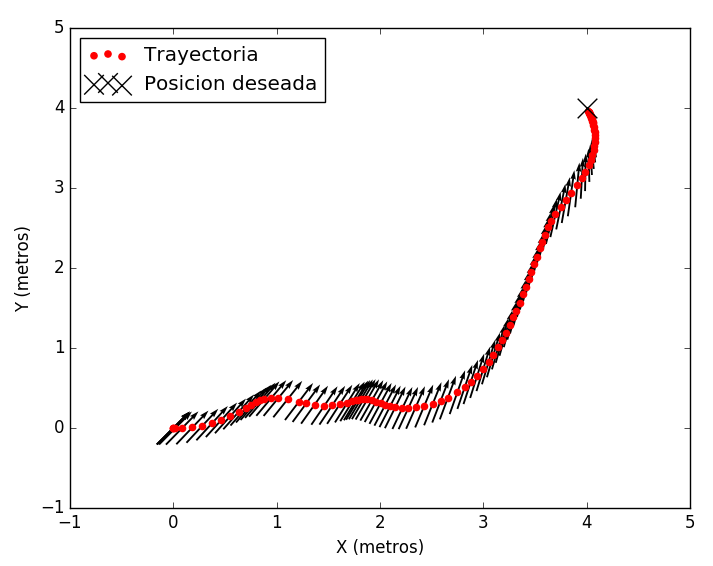
\includegraphics[width=0.61\textwidth]{images/attr_kbki.png}
%  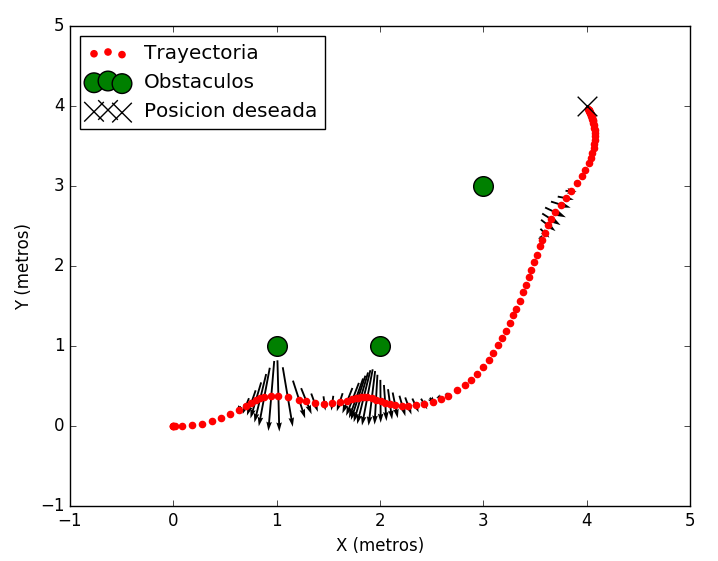
\includegraphics[width=0.60\textwidth]{images/rep_kbki.png}
%  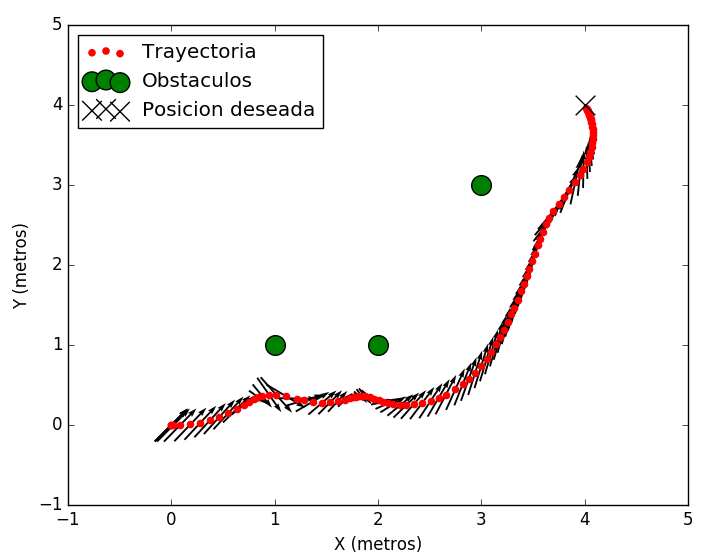
\includegraphics[width=0.60\textwidth]{images/nav_kbki.png}
%  \captionsetup{font=footnotesize}
%  \caption{Navegación autónoma implementada en el robot diferencial Kobuki.}
%  \label{f:kbki_APF}
%\end{figure}
La metodología propuesta se implementó como un algoritmo iterativo en el robot Kobuki. 
Como se se describe en la sección \ref{sec:autonomia}, el algoritmo toma iterativamente 
posiciones deseadas  donde a través del campo potencial artificial y el controlador 
polar impulsan al robot a través de las posiciones requeridas. Se expuso al robot 
a diferentes obstáculos cuyas posiciones fueron conocidas a priori. La figura 
\ref{f:kbki_APF} (a) muestra las fuerzas de atracción para cada posición (puntos rojos) en 
las que el algoritmo se itera en el entorno de dos dimensiones dentro del movimiento del 
robot. Para cada posición, el campo de potencial atractivo que se puede ver con la dirección 
de las flechas. La figura \ref{f:kbki_APF} (b) se compone de las fuerzas de repulsión basadas en 
los obstáculos, que se muestran como marcadores verdes. Para cada obstáculo, la magnitud de 
las fuerzas aumenta cuando el robot está más cerca y su dirección señala los obstáculos, permitiendo 
que el robot los evite. La figura \ref{f:kbki_APF} (c) muestra la superposición de ambas fuerzas 
con los obstáculos reales. Cada fuerza proporciona una posición deseada intermedia para el 
robot, que constituye la posición deseada continuamente actualizada para el controlador 
polar. Aunque las fuerzas cercanas a los obstáculos tienen un alto índice de cambio, la 
trayectoria es suave. Esto demuestra la efectividad del controlador polar a pesar de las 
características no holonómicas del robot.

\section{Resultados de la Navegación Autónoma con el Lidar (2D)}
\begin{figure}%[ht!]
  \centering \footnotesize
  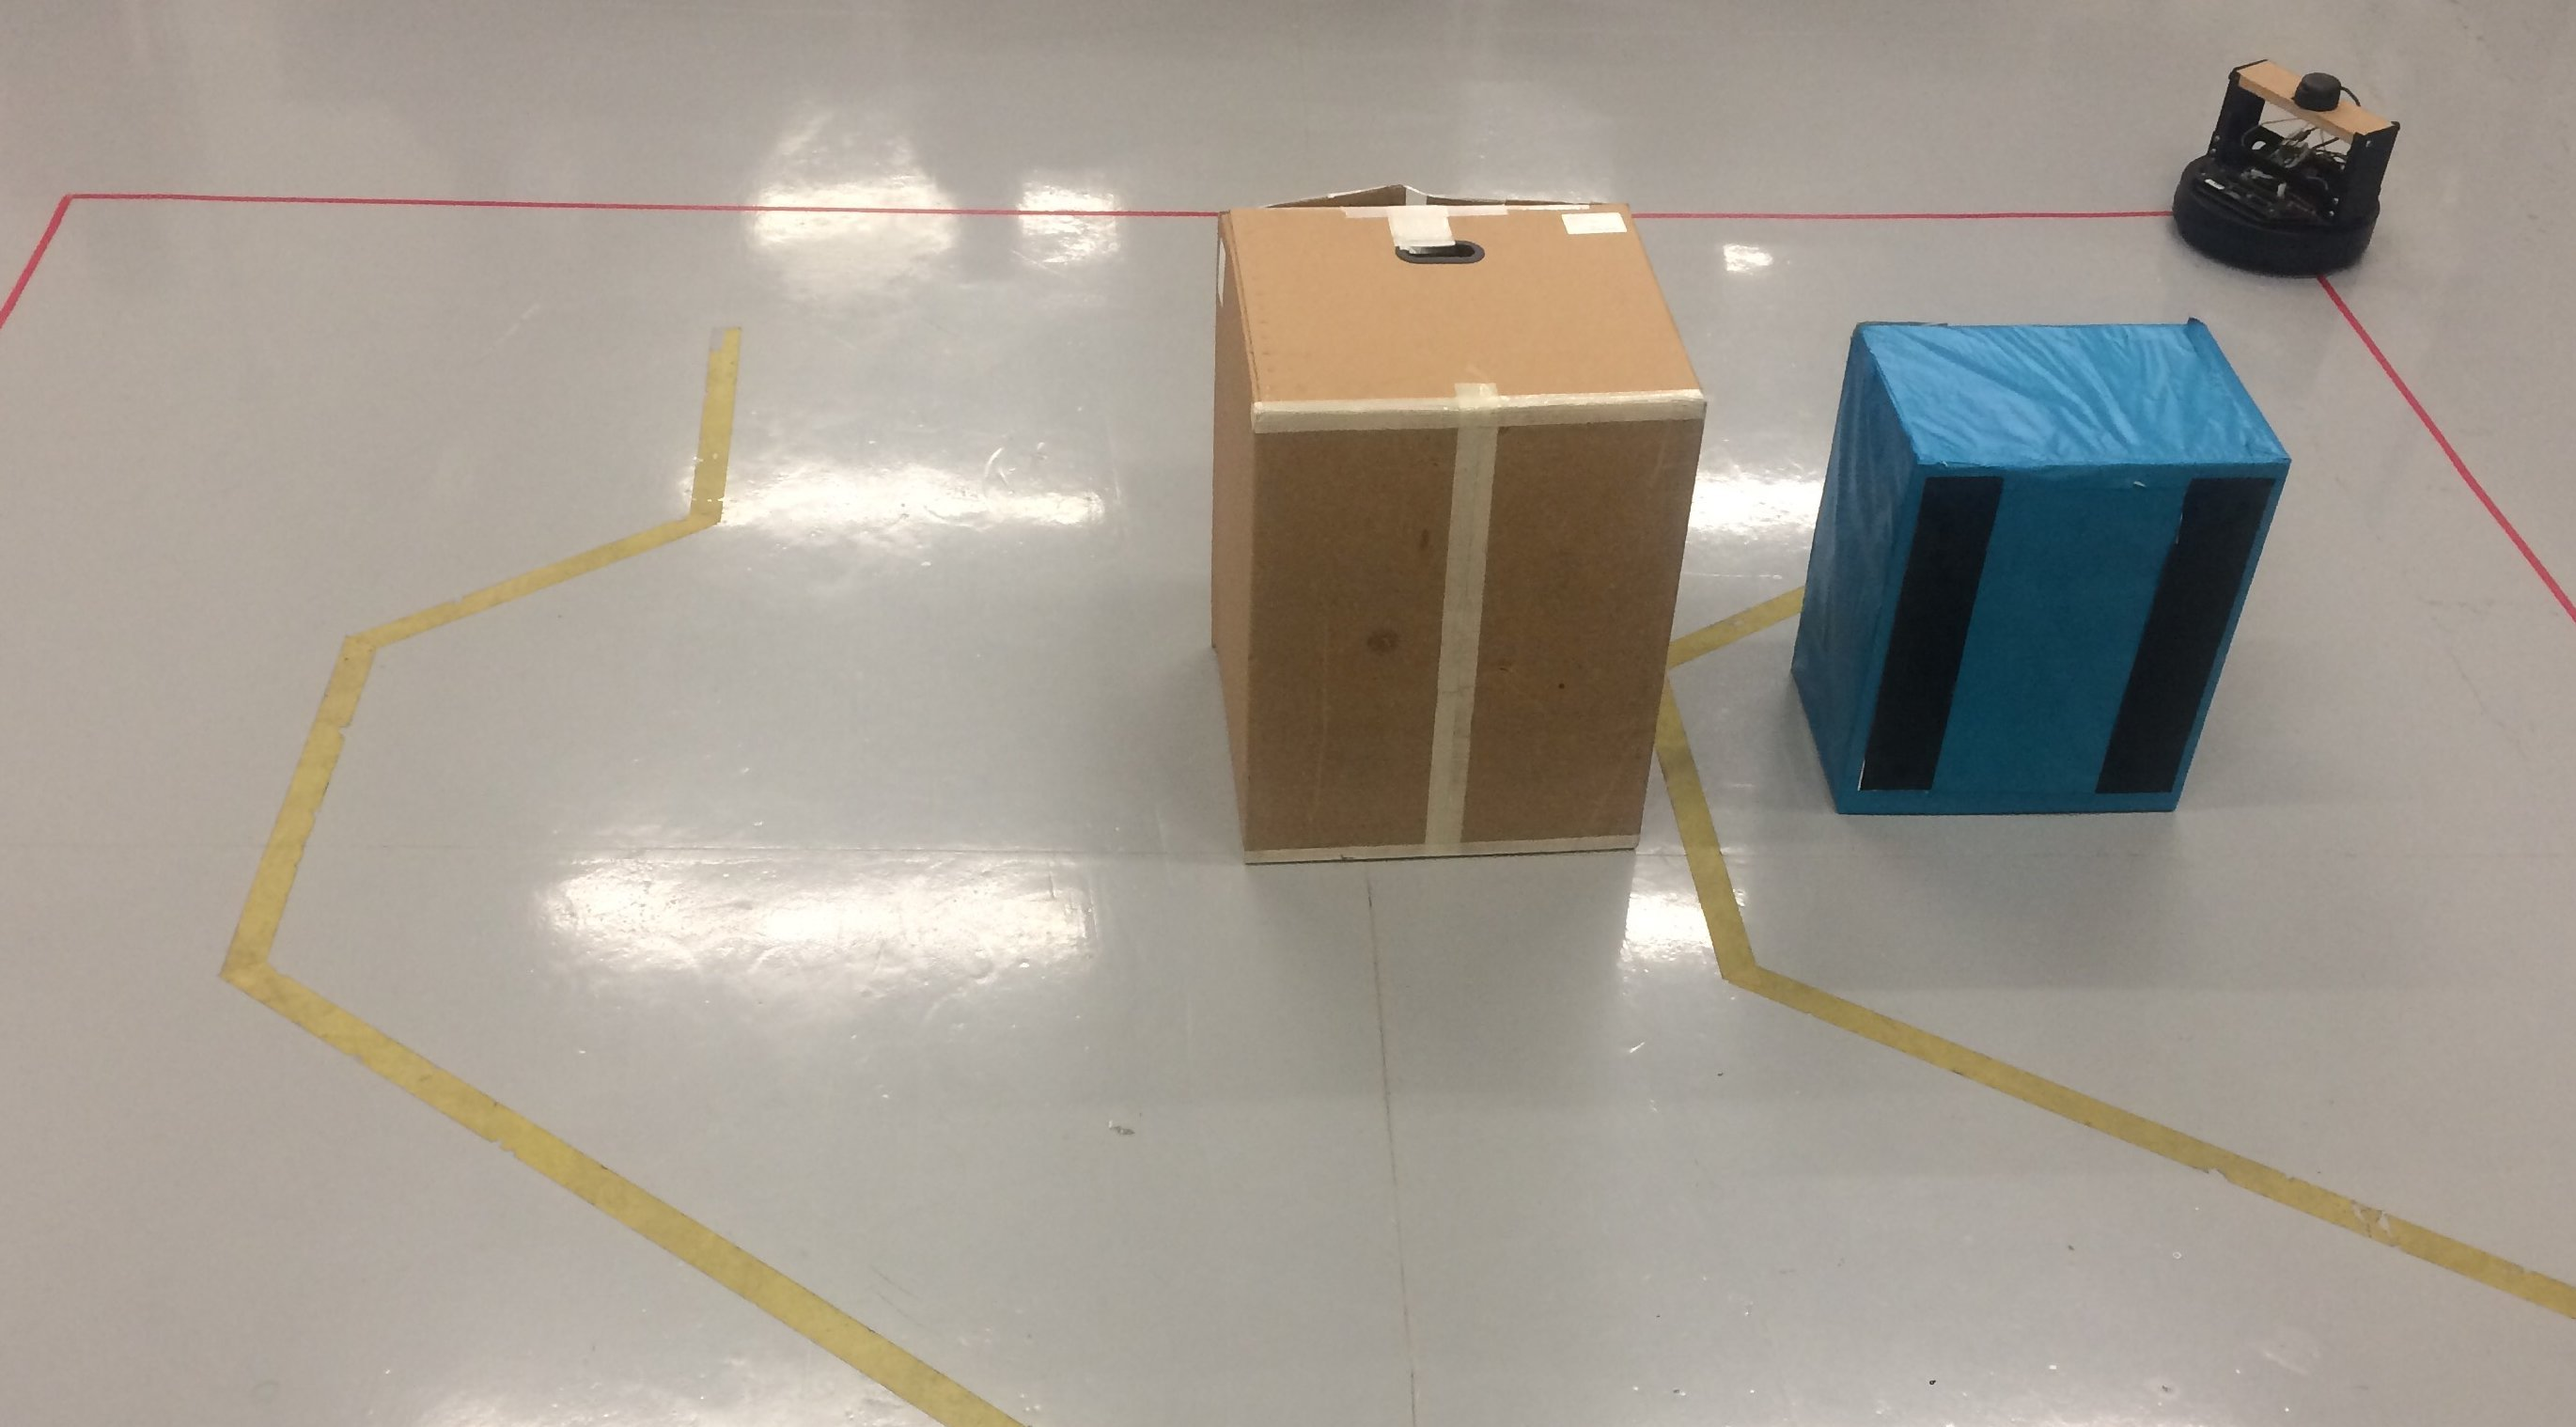
\includegraphics[width=0.80\textwidth]{images/kobuki_201.jpg}
  \captionsetup{font=footnotesize}
  \caption{Navegación autónoma del Kobuki montado un sensor lidar y dos cajas
  como obstáculos}
\end{figure}

\begin{figure}[ht!]
     \begin{center}
        \subfigure[Fuerzas de atracción aplicado al robot móvil]{\label{fig:etiquetaA}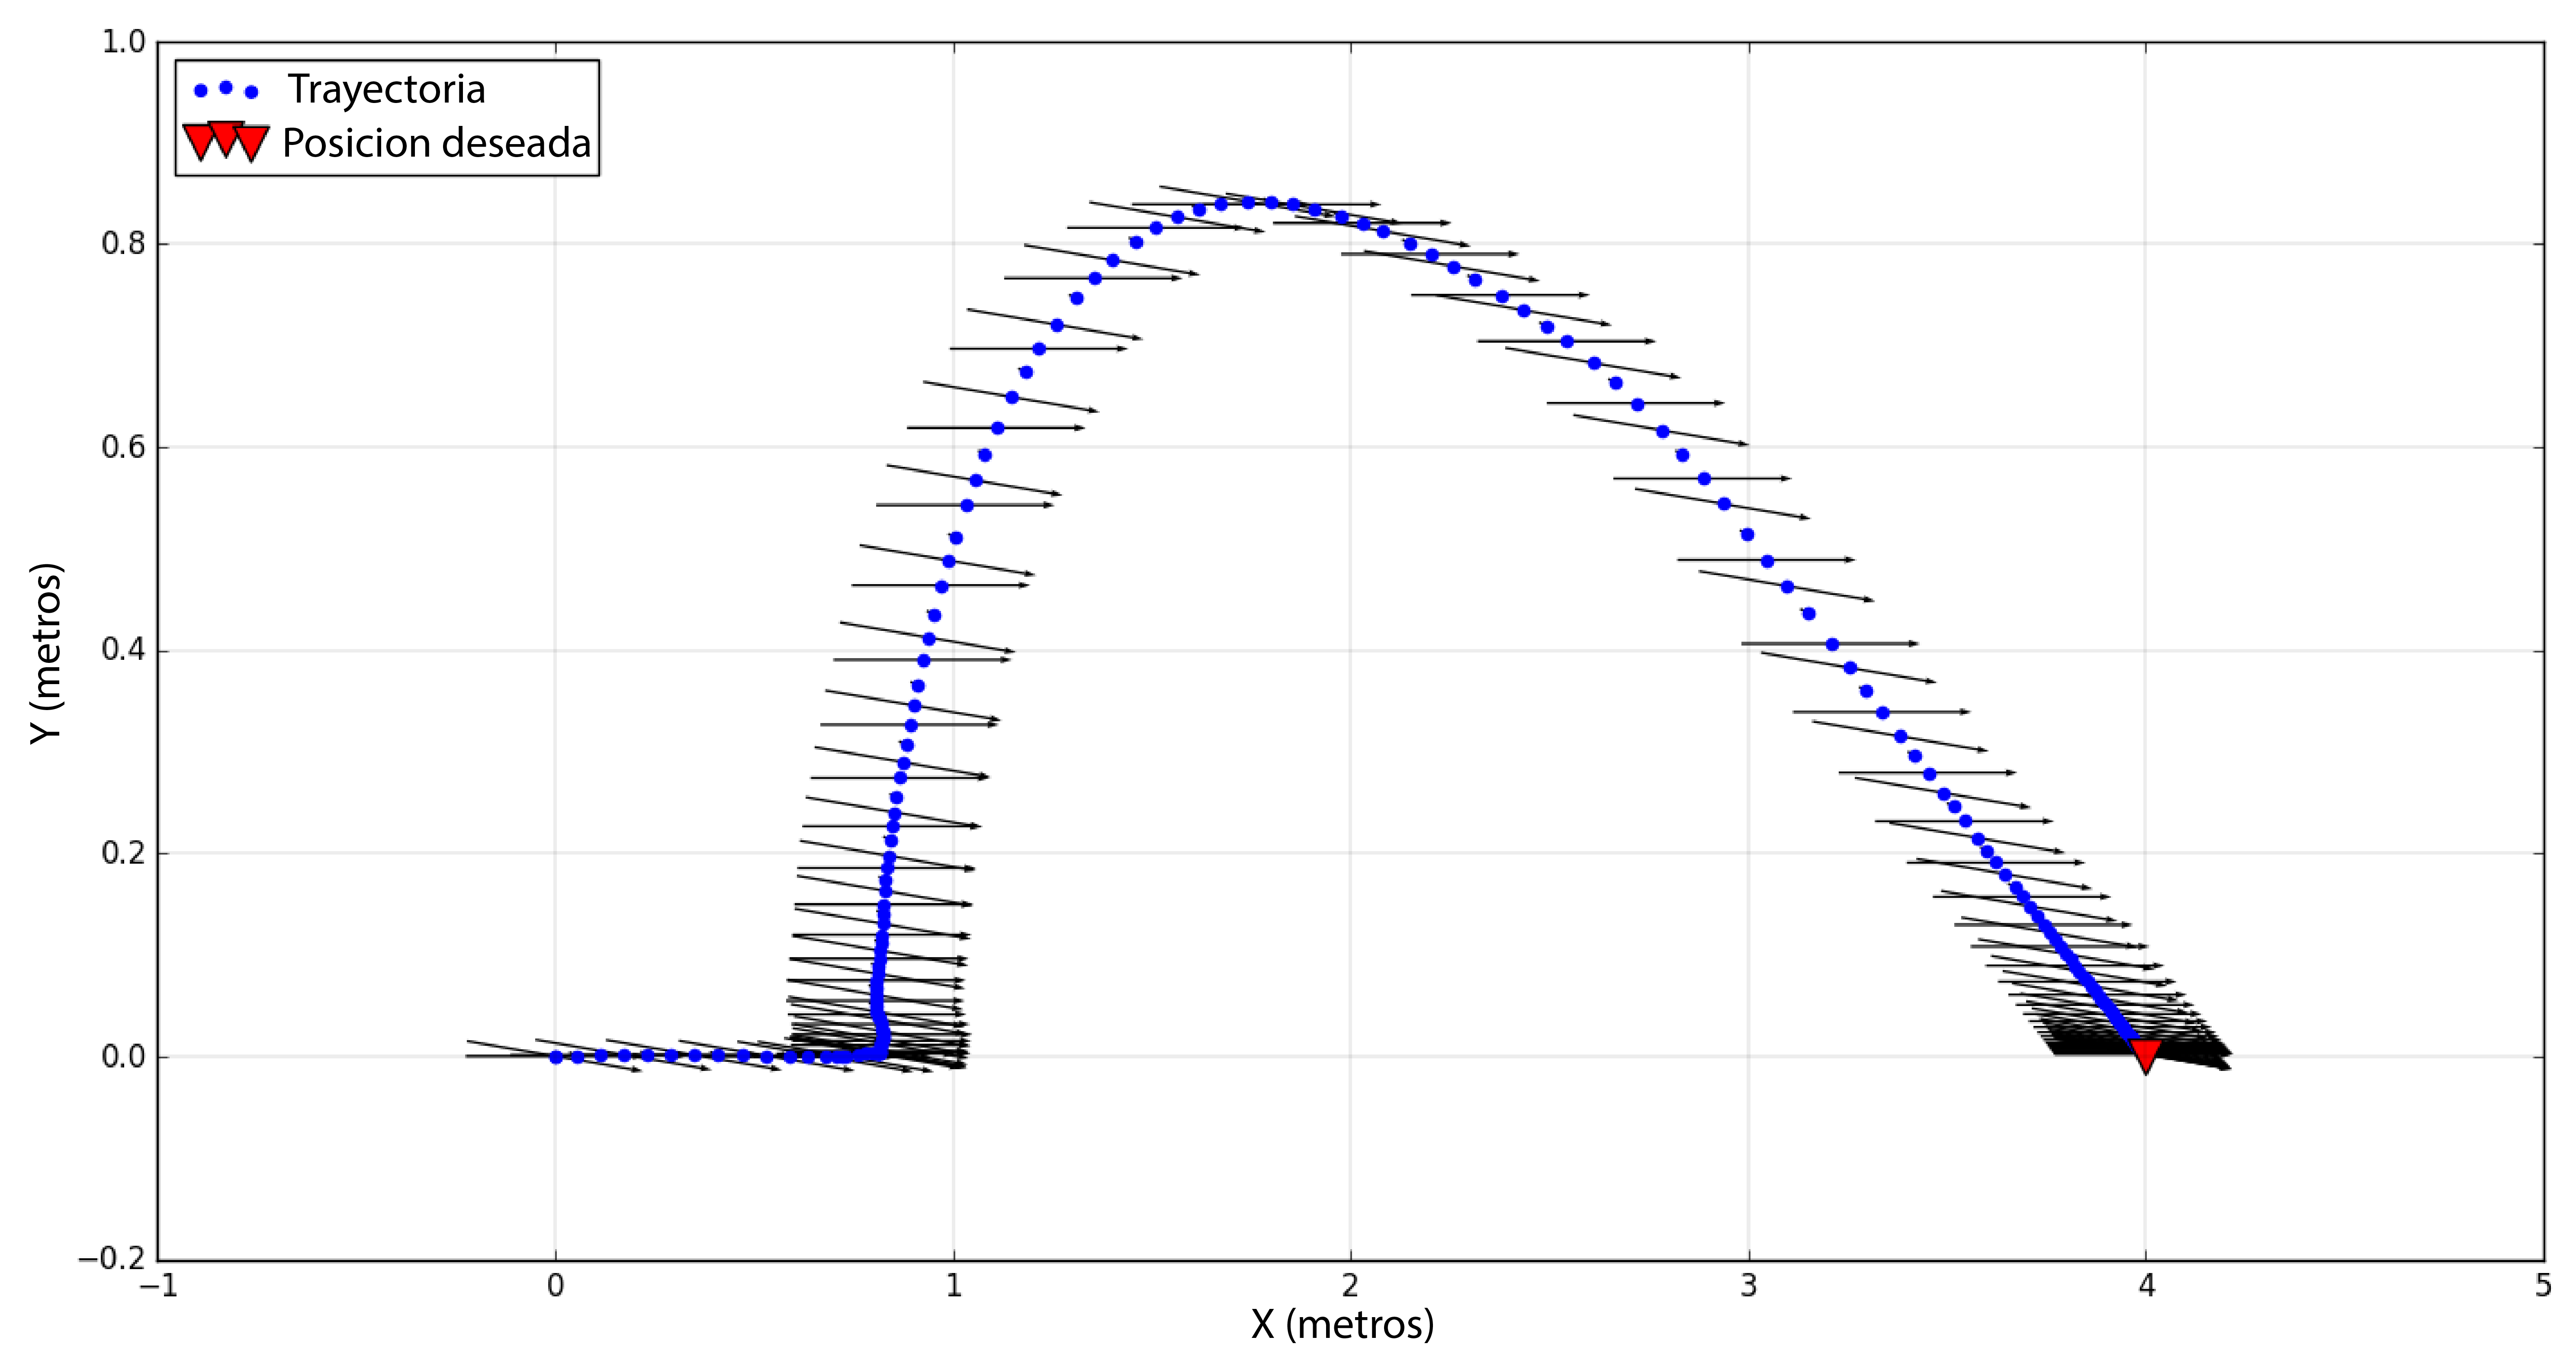
\includegraphics
        [width=.69\textwidth]{images/fattr_lidar_s.png}}
        \subfigure[Fuerzas de repulsión aplicado al robot móvil]{\label{fig:etiquetaB}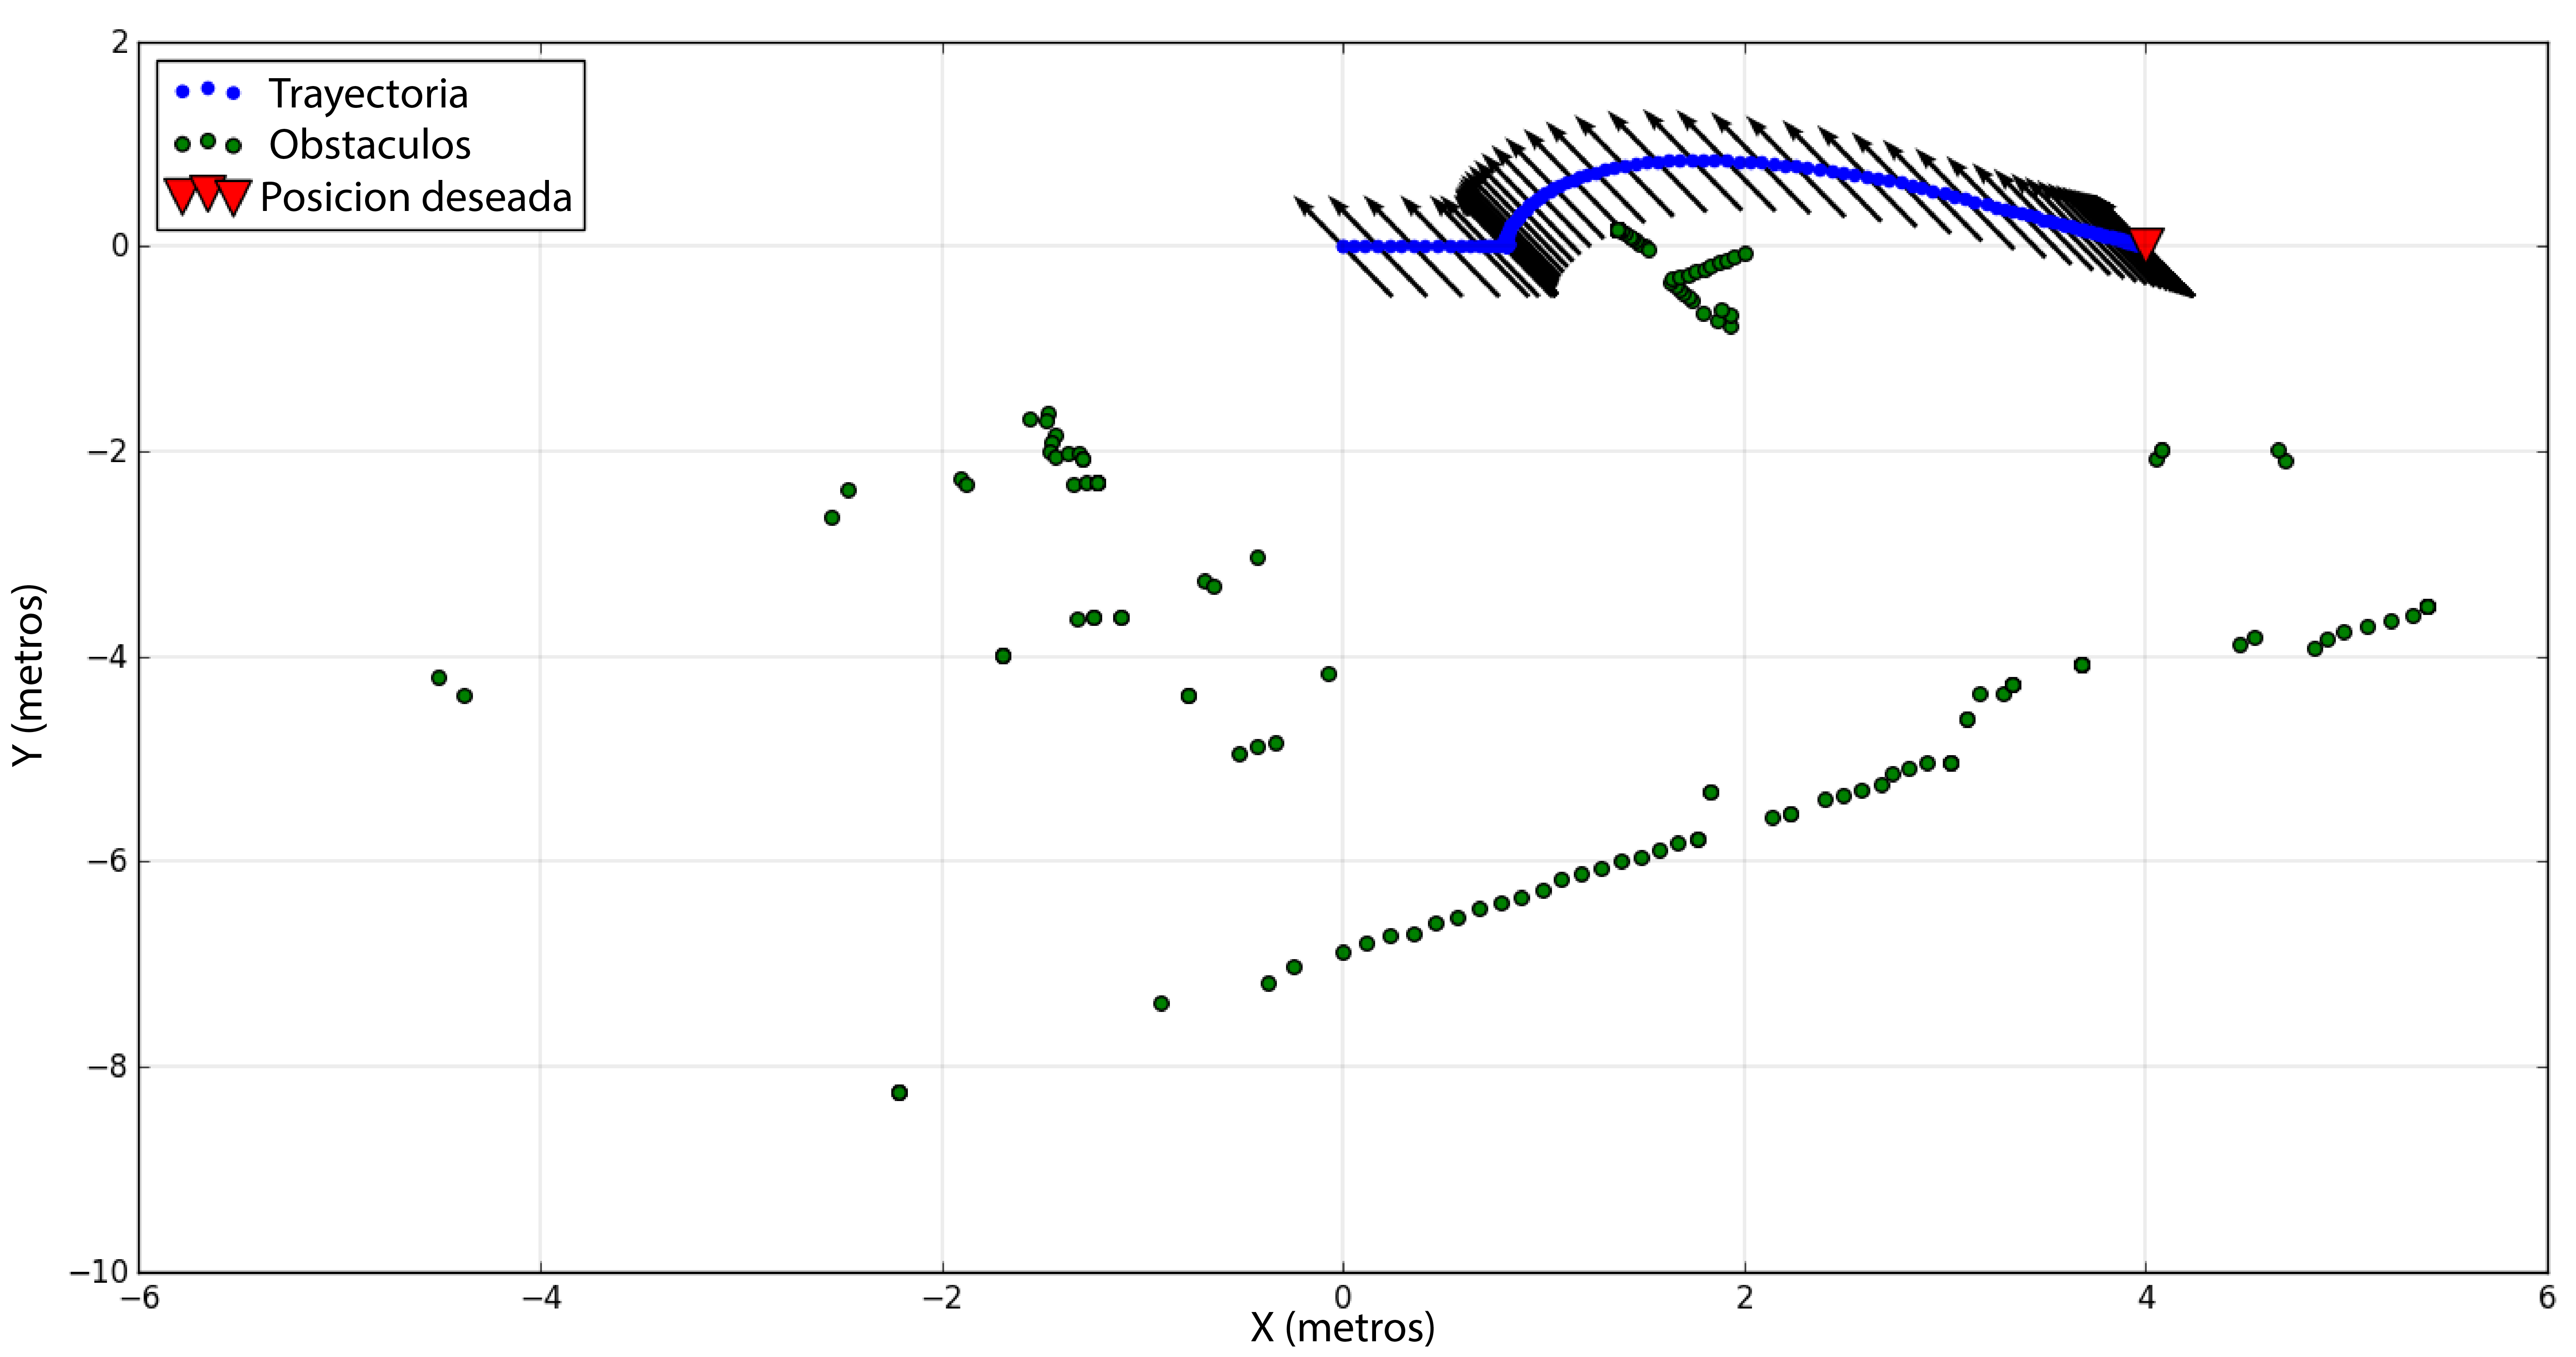
\includegraphics
        [width=.69\textwidth]{images/frep_lidar_s.png}}
        \subfigure[Fuerzas de navegación aplicado al robot móvil]{\label{fig:etiquetaC}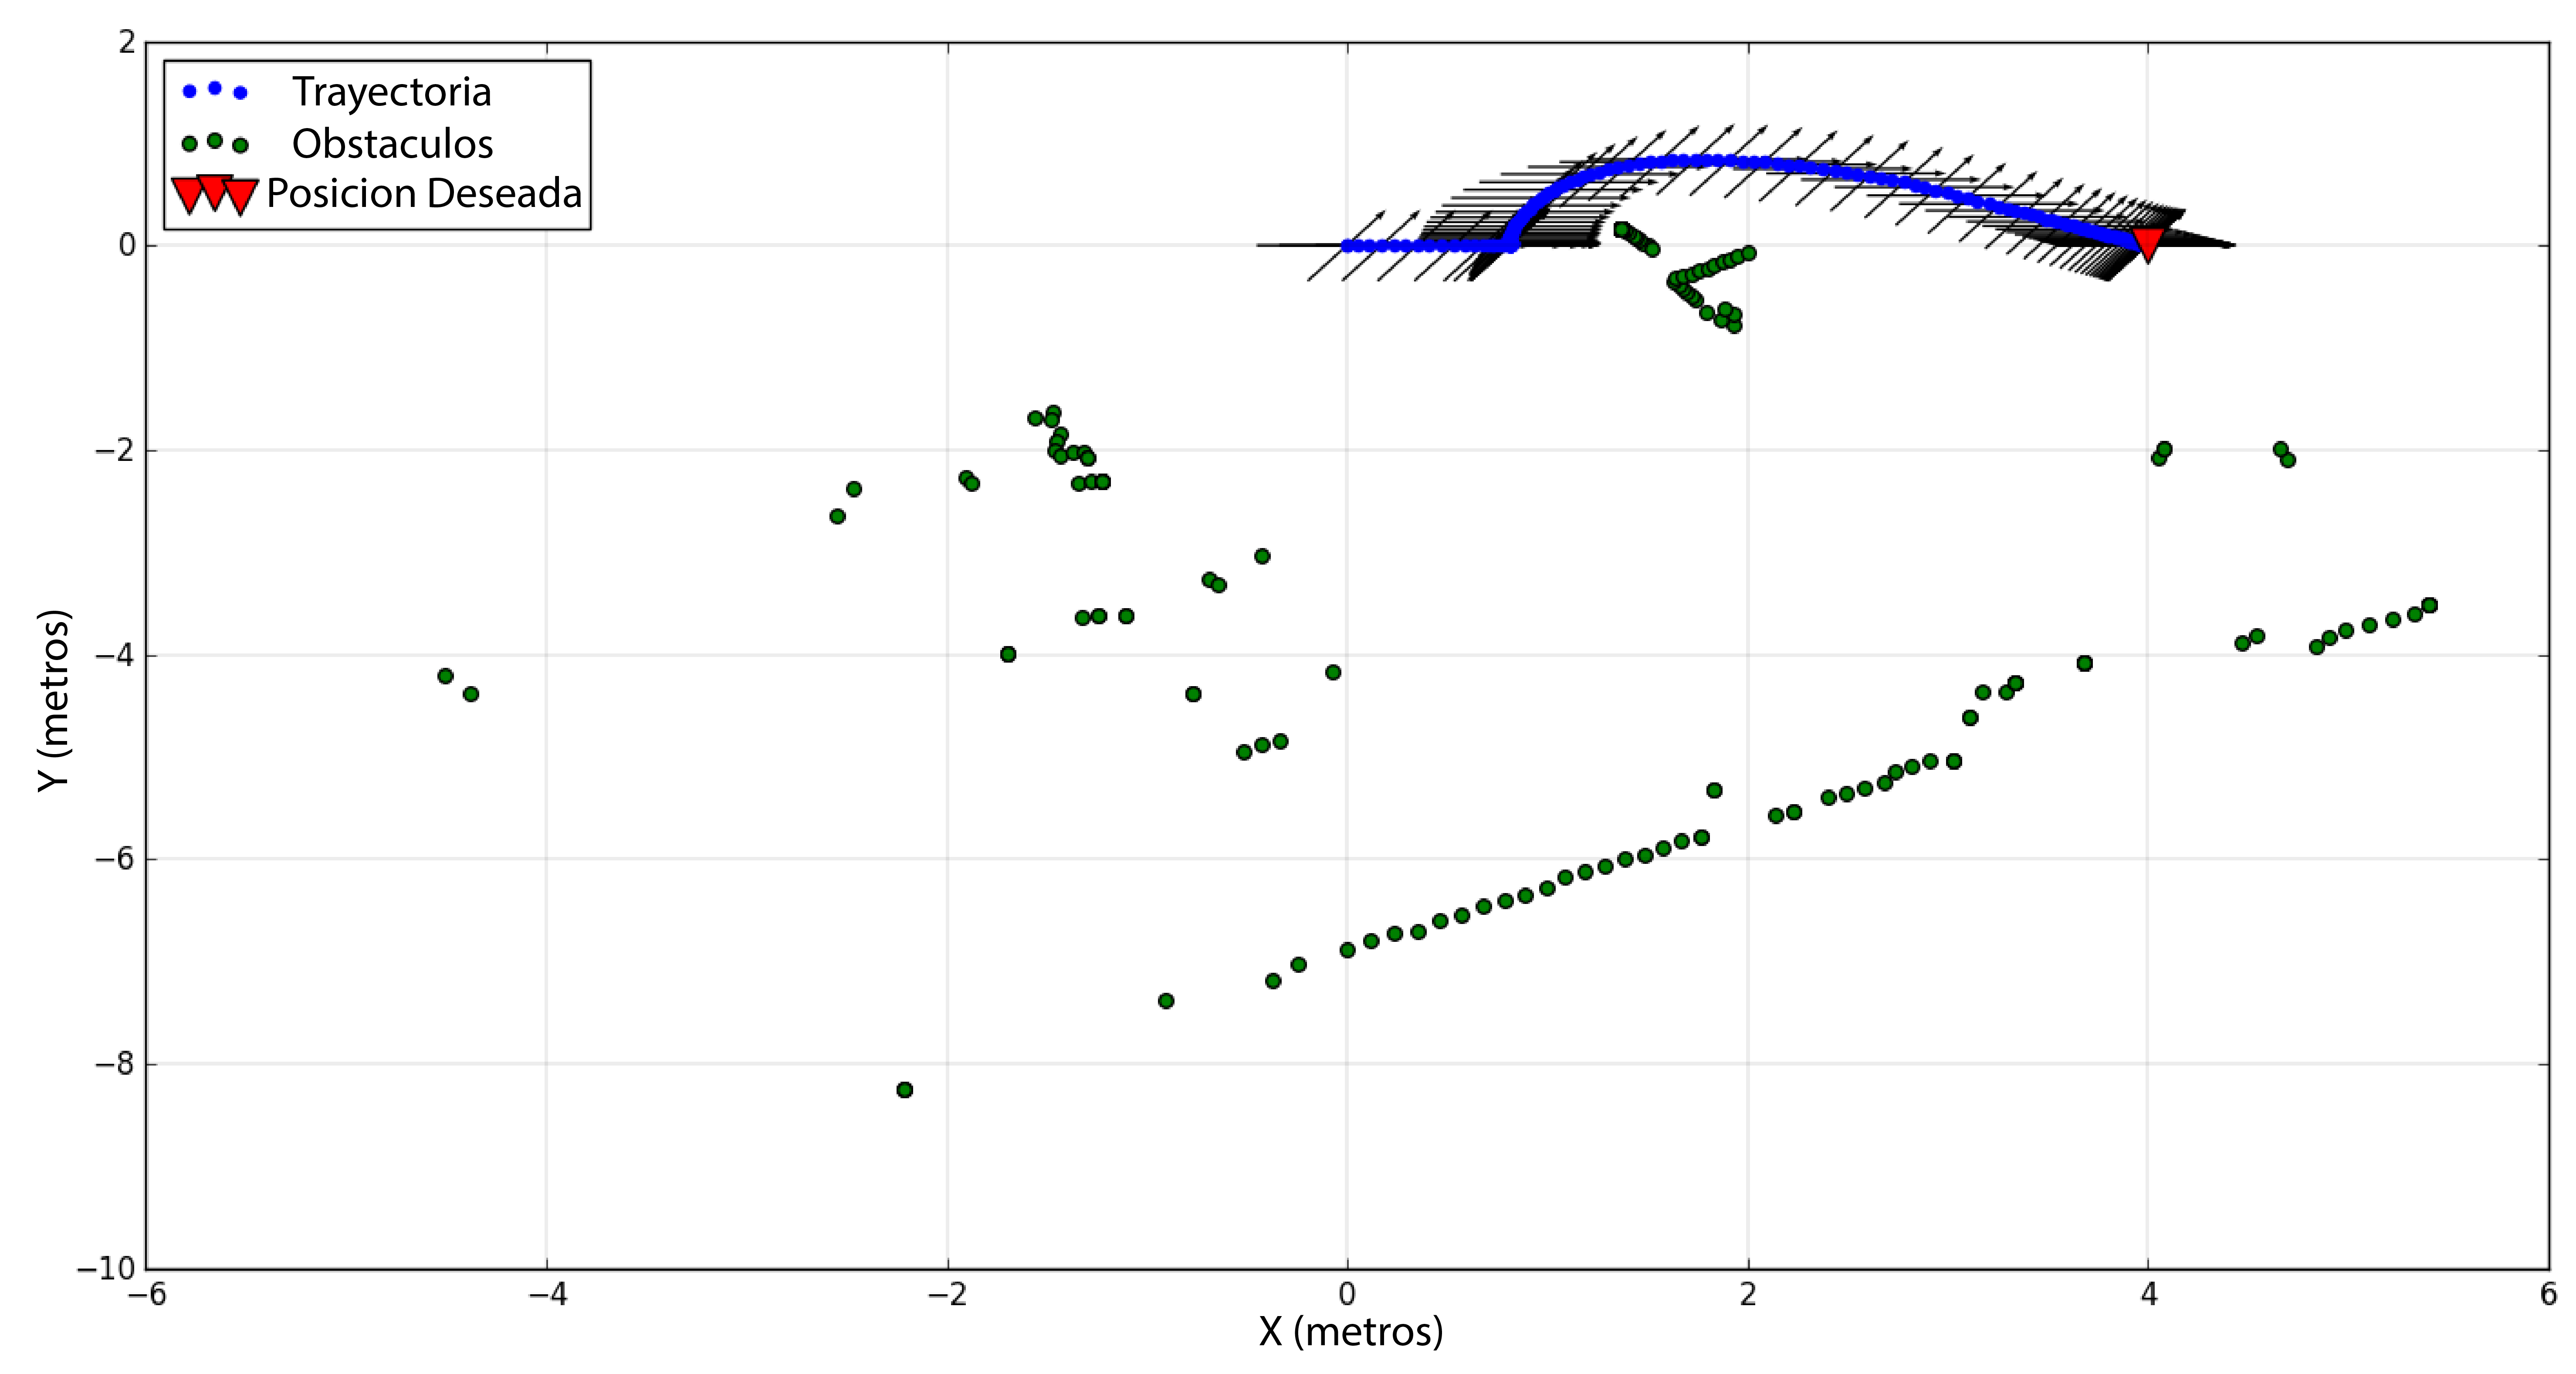
\includegraphics
        [width=.69\textwidth]{images/fnav_lidar_s.png}}
    \end{center}
  \captionsetup{font=footnotesize}
    \caption{\label{f:kbki_autonomo}Campos atractivos y repulsivos, y la trayectoria que el robot real sigue 
  usando datos en línea provenientes del sensor lidar montado en la parte superior.}
\end{figure}

%\begin{figure}%[ht!]
%  \centering \footnotesize
%  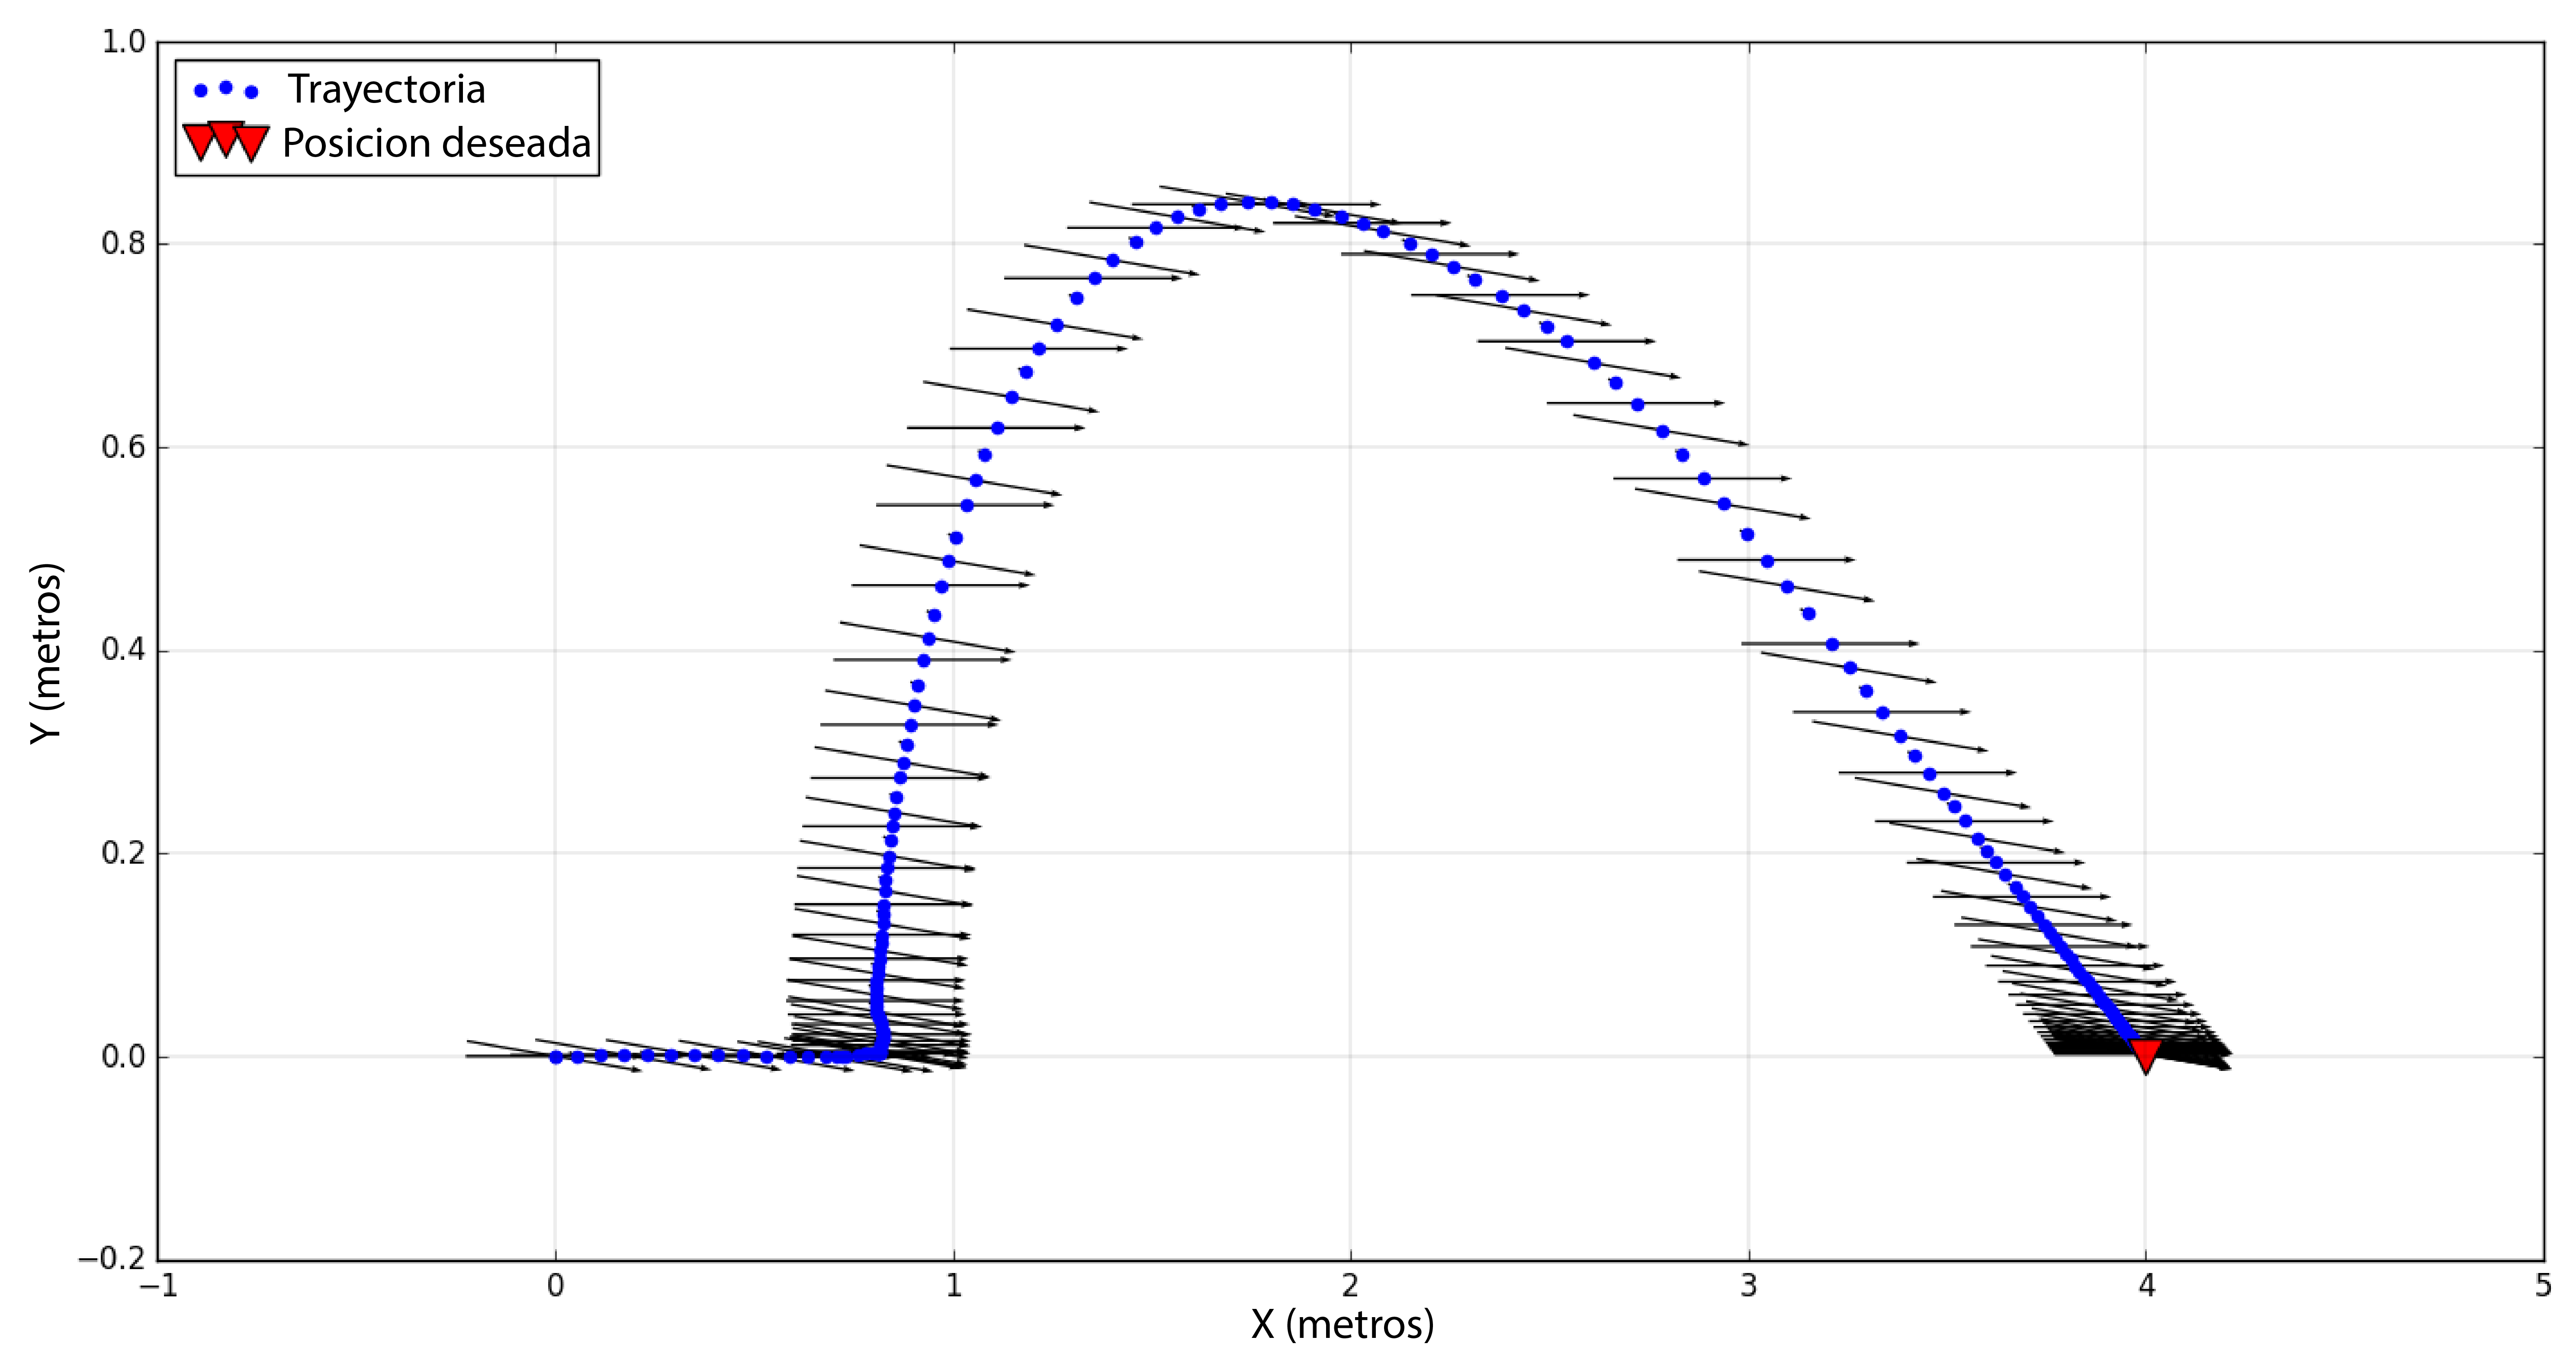
\includegraphics[width=0.80\textwidth]{images/fattr_lidar_s.png}
%  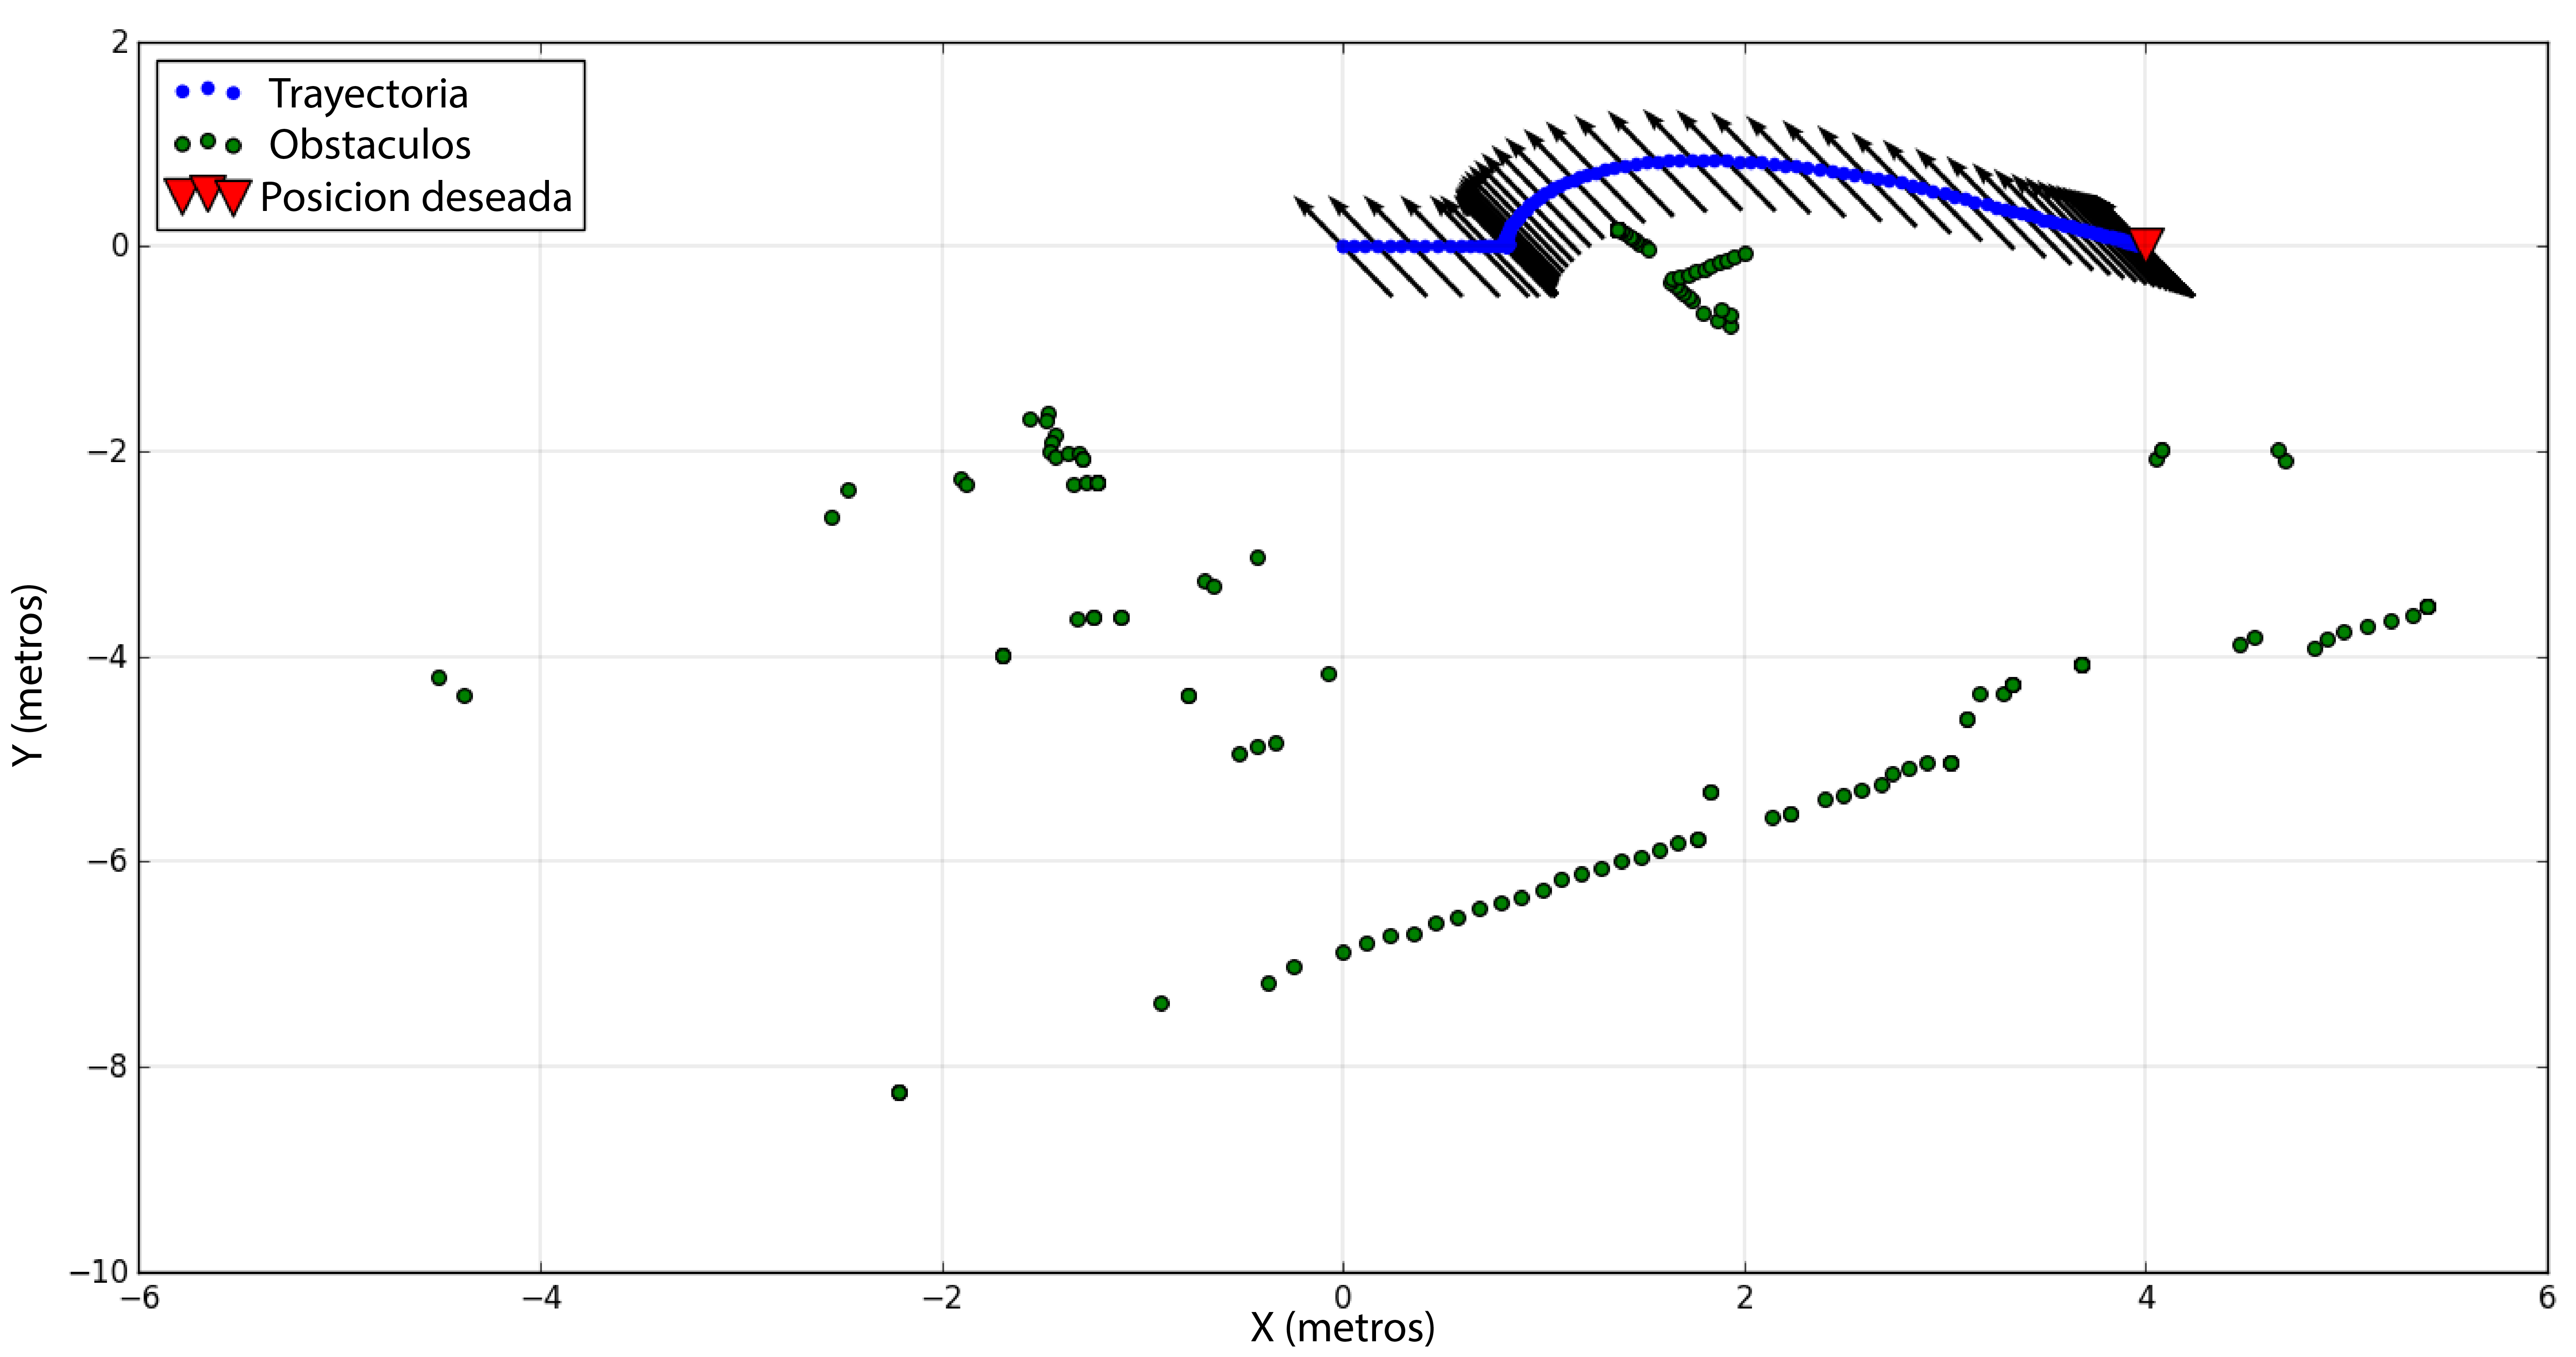
\includegraphics[width=0.80\textwidth]{images/frep_lidar_s.png}
%  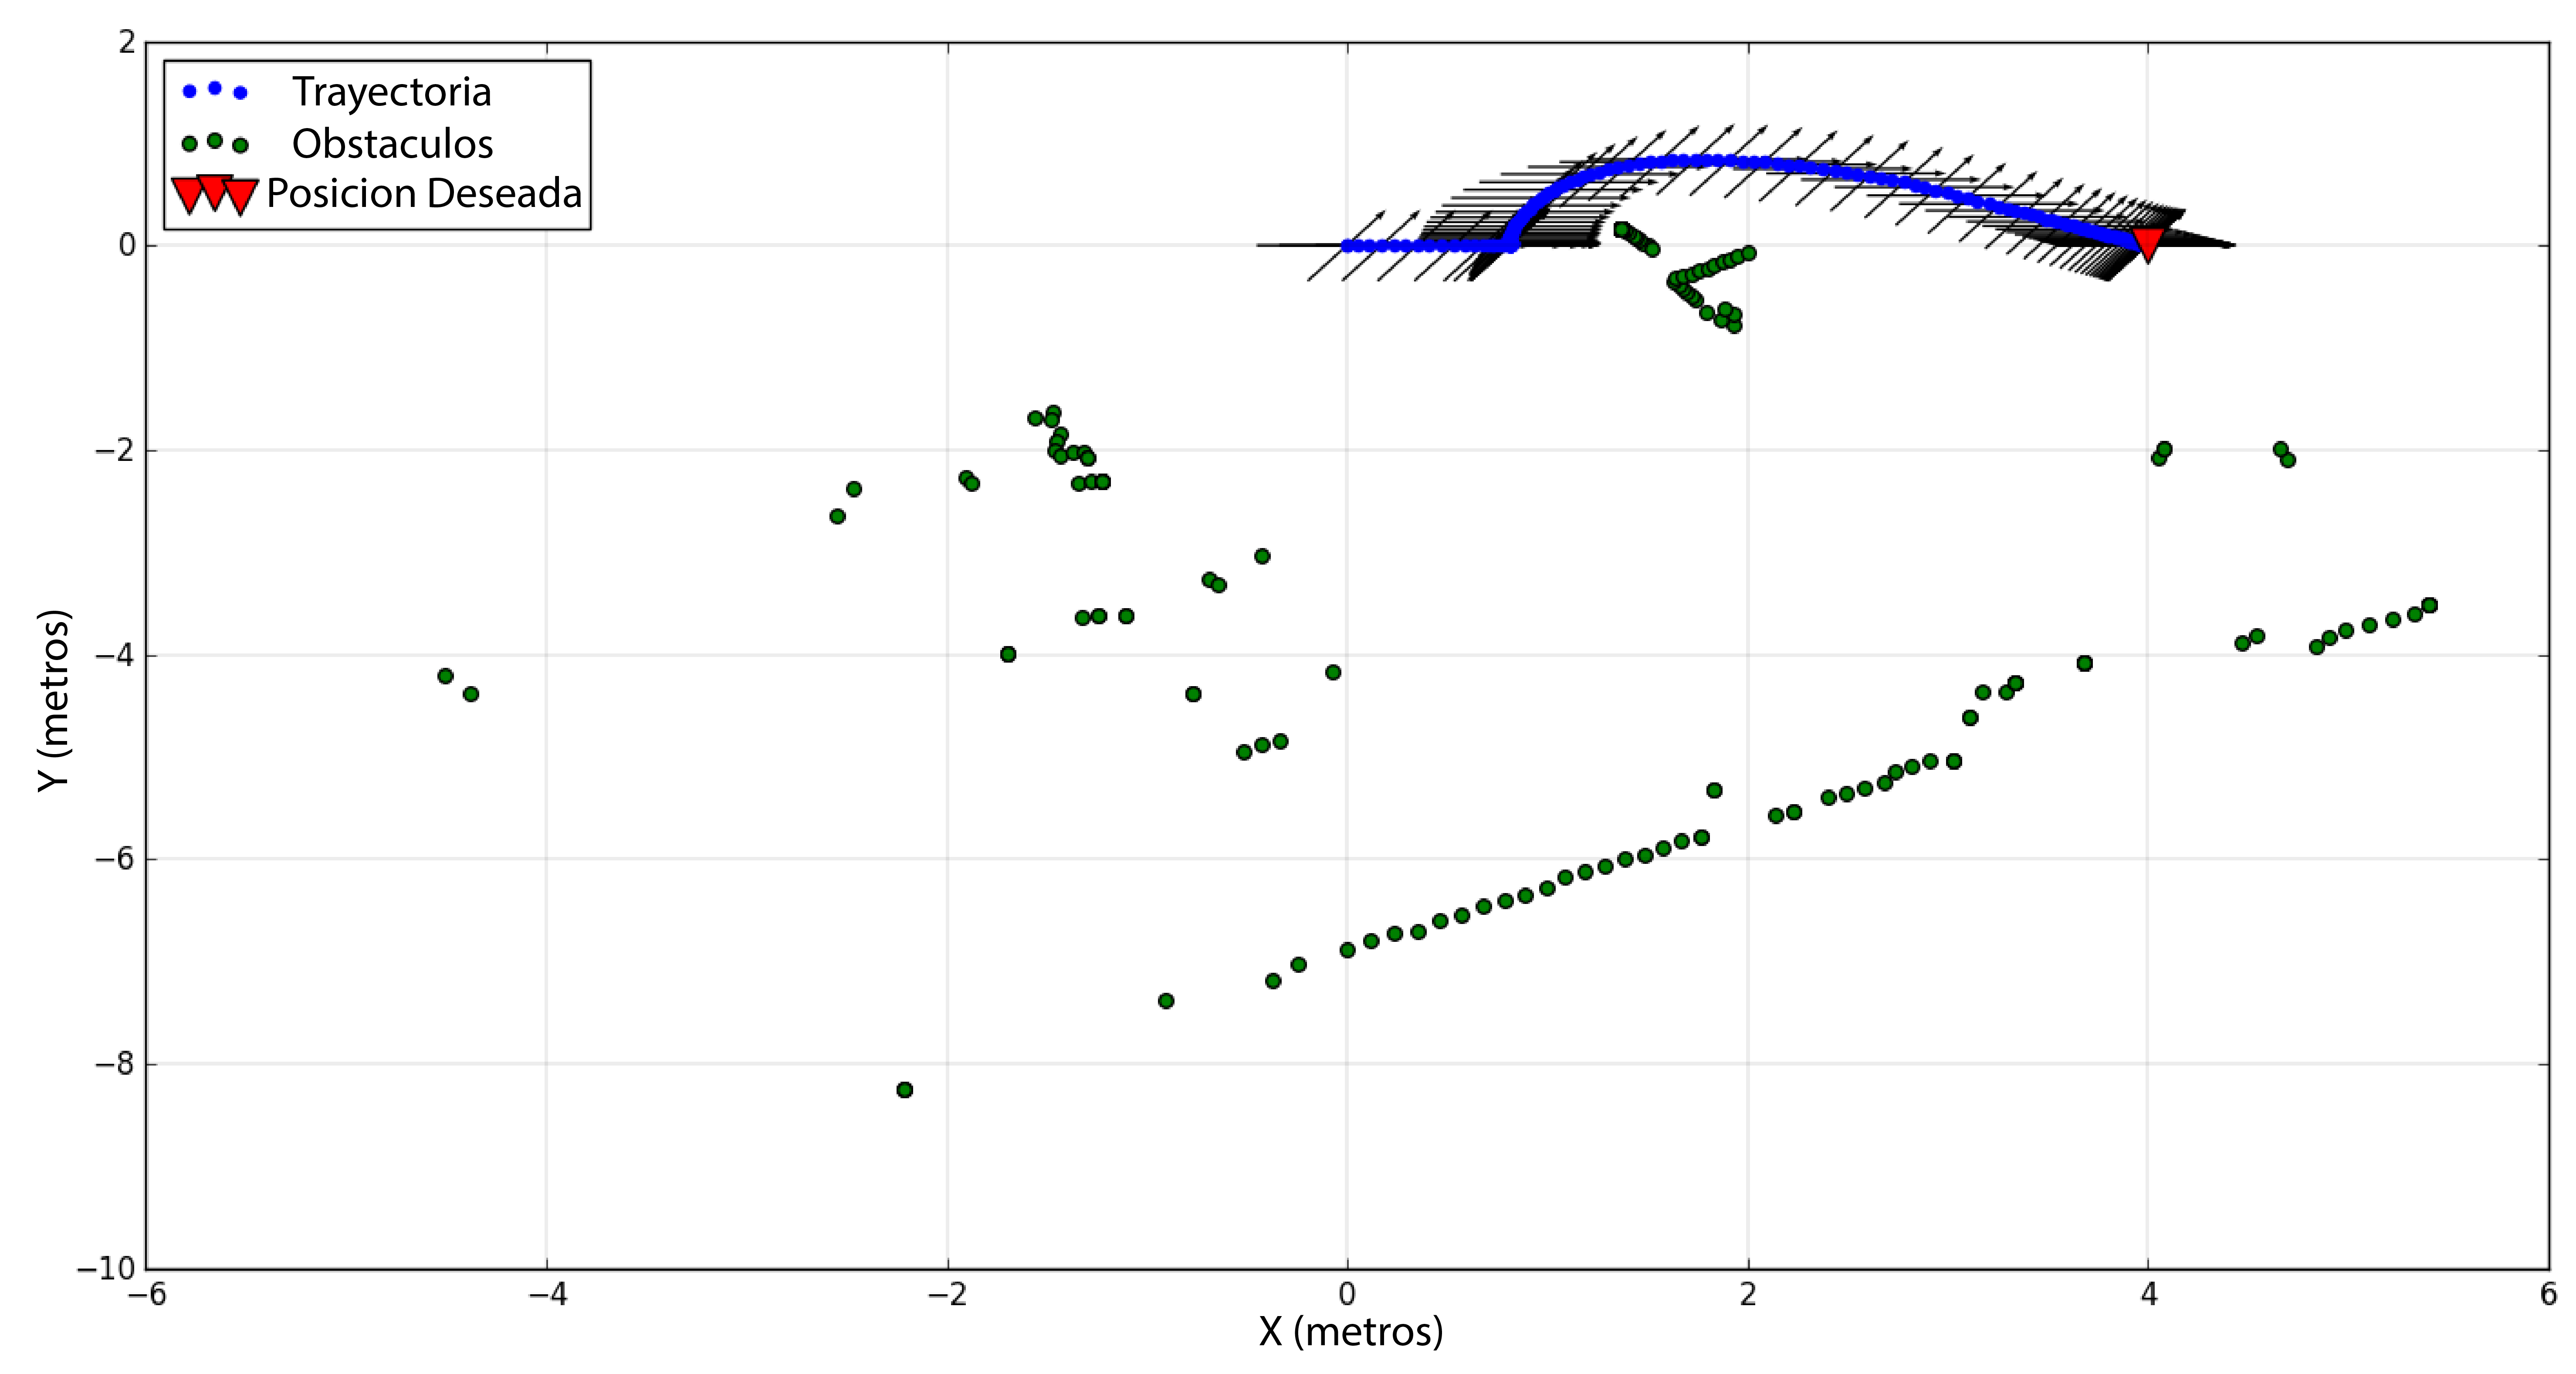
\includegraphics[width=0.80\textwidth]{images/fnav_lidar_s.png}
%  \captionsetup{font=footnotesize}
%  \caption{Campos atractivos y repulsivos, y la trayectoria que el robot real sigue 
%  usando datos en línea provenientes del sensor lidar montado en la parte superior.}
%  \label{f:kbki_autonomo}
%\end{figure}

Para probar la autonomía del robot móvil en un entorno real, se usa un sensor lidar 
(RPLidar A2) que se colocó sobre el robot Kobuki. Se usa el sensor lidar para poder 
hacer una actualización continua de las posiciones de los obstáculos a medida que el 
robot se mueve. El robot usa tópicos creados en ROS para obtener la información del 
sensor que se compone del rango y la orientación de cada punto medido, a medida que 
el lidar gira. La información del lidar se tuvo que convertir a coordenadas cartesianas 
para conocer las posiciones cartesianas de los obstáculos dentro del espacio de trabajo, 
que es la entrada al algoritmo principal. Para que el kobuki pueda moverse dentro del 
mapa generado por el lidar, el marco de referencia del robot se tomó como el marco del 
lidar. Entonces, el algoritmo de navegación autónomo usa las coordenadas del obstáculo 
para generar su propia trayectoria evitando obstáculos. Para toda la prueba, se colocaron 
dos cajas en el espacio de trabajo, como se ve en la figura \ref{f:kbki_autonomo} (a). La 
posición del objetivo era ($x = 4, y = 0$). La figura \ref{f:kbki_autonomo} (b) muestra 
la trayectoria del robot en azul y las flechas que indican la fuerza que lleva al robot a la 
posición deseada. La figura \ref{f:kbki_autonomo} (c) muestra el mapa completo, donde los 
puntos verdes representan el entorno, detectados por el lidar, donde se mueve el robot. Como 
se observa, estas flechas apuntan hacia afuera del obstáculo, proporcionando autonomía al 
robot mientras intenta alcanzar la posición deseada. Finalmente en la figura 
\ref{f:kbki_autonomo} (d) se muestra toda la fuerza de navegación que impulsa el movimiento 
del robot móvil.

\section{Resultado de la autonomía del robot junto al SLAM}
\begin{figure}%[ht!]
  \centering \footnotesize
  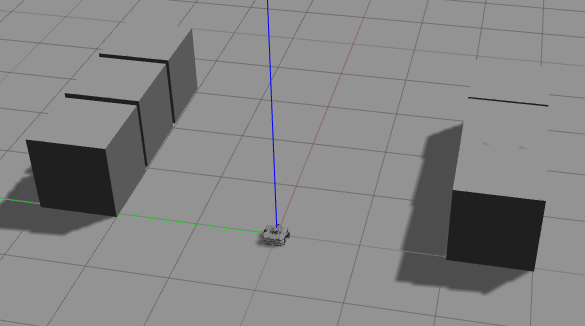
\includegraphics[width=0.80\textwidth]{images/gazebo_map.png}
  \captionsetup{font=footnotesize}
  \caption{Mapa en Gazebo}
  \label{fig:Gazebo_simu}
\end{figure}
Para probar la autonomía del robot junto con el algoritmo SLAM, se uso un simulador dinámico 
en Gazebo con el robot Kobuki con obstáculos. Los obstáculos fueron colocados de tal manera
que pueda representar la entrada de un túnel. Esto se muestra en la figura 
\ref{fig:Gazebo_simu}. El túnel tiene un ancho de 4 metros y un largo de 3 metros por donde 
el robot se va a desplazar, estimar la posición de los obstáculos y construir el mapa en dos 
dimensiones.

\begin{figure}[ht!]
     \begin{center}
        \subfigure[Fuerzas de atracción aplicado al robot móvil en tiempo real]{\label{fig:etiquetaA}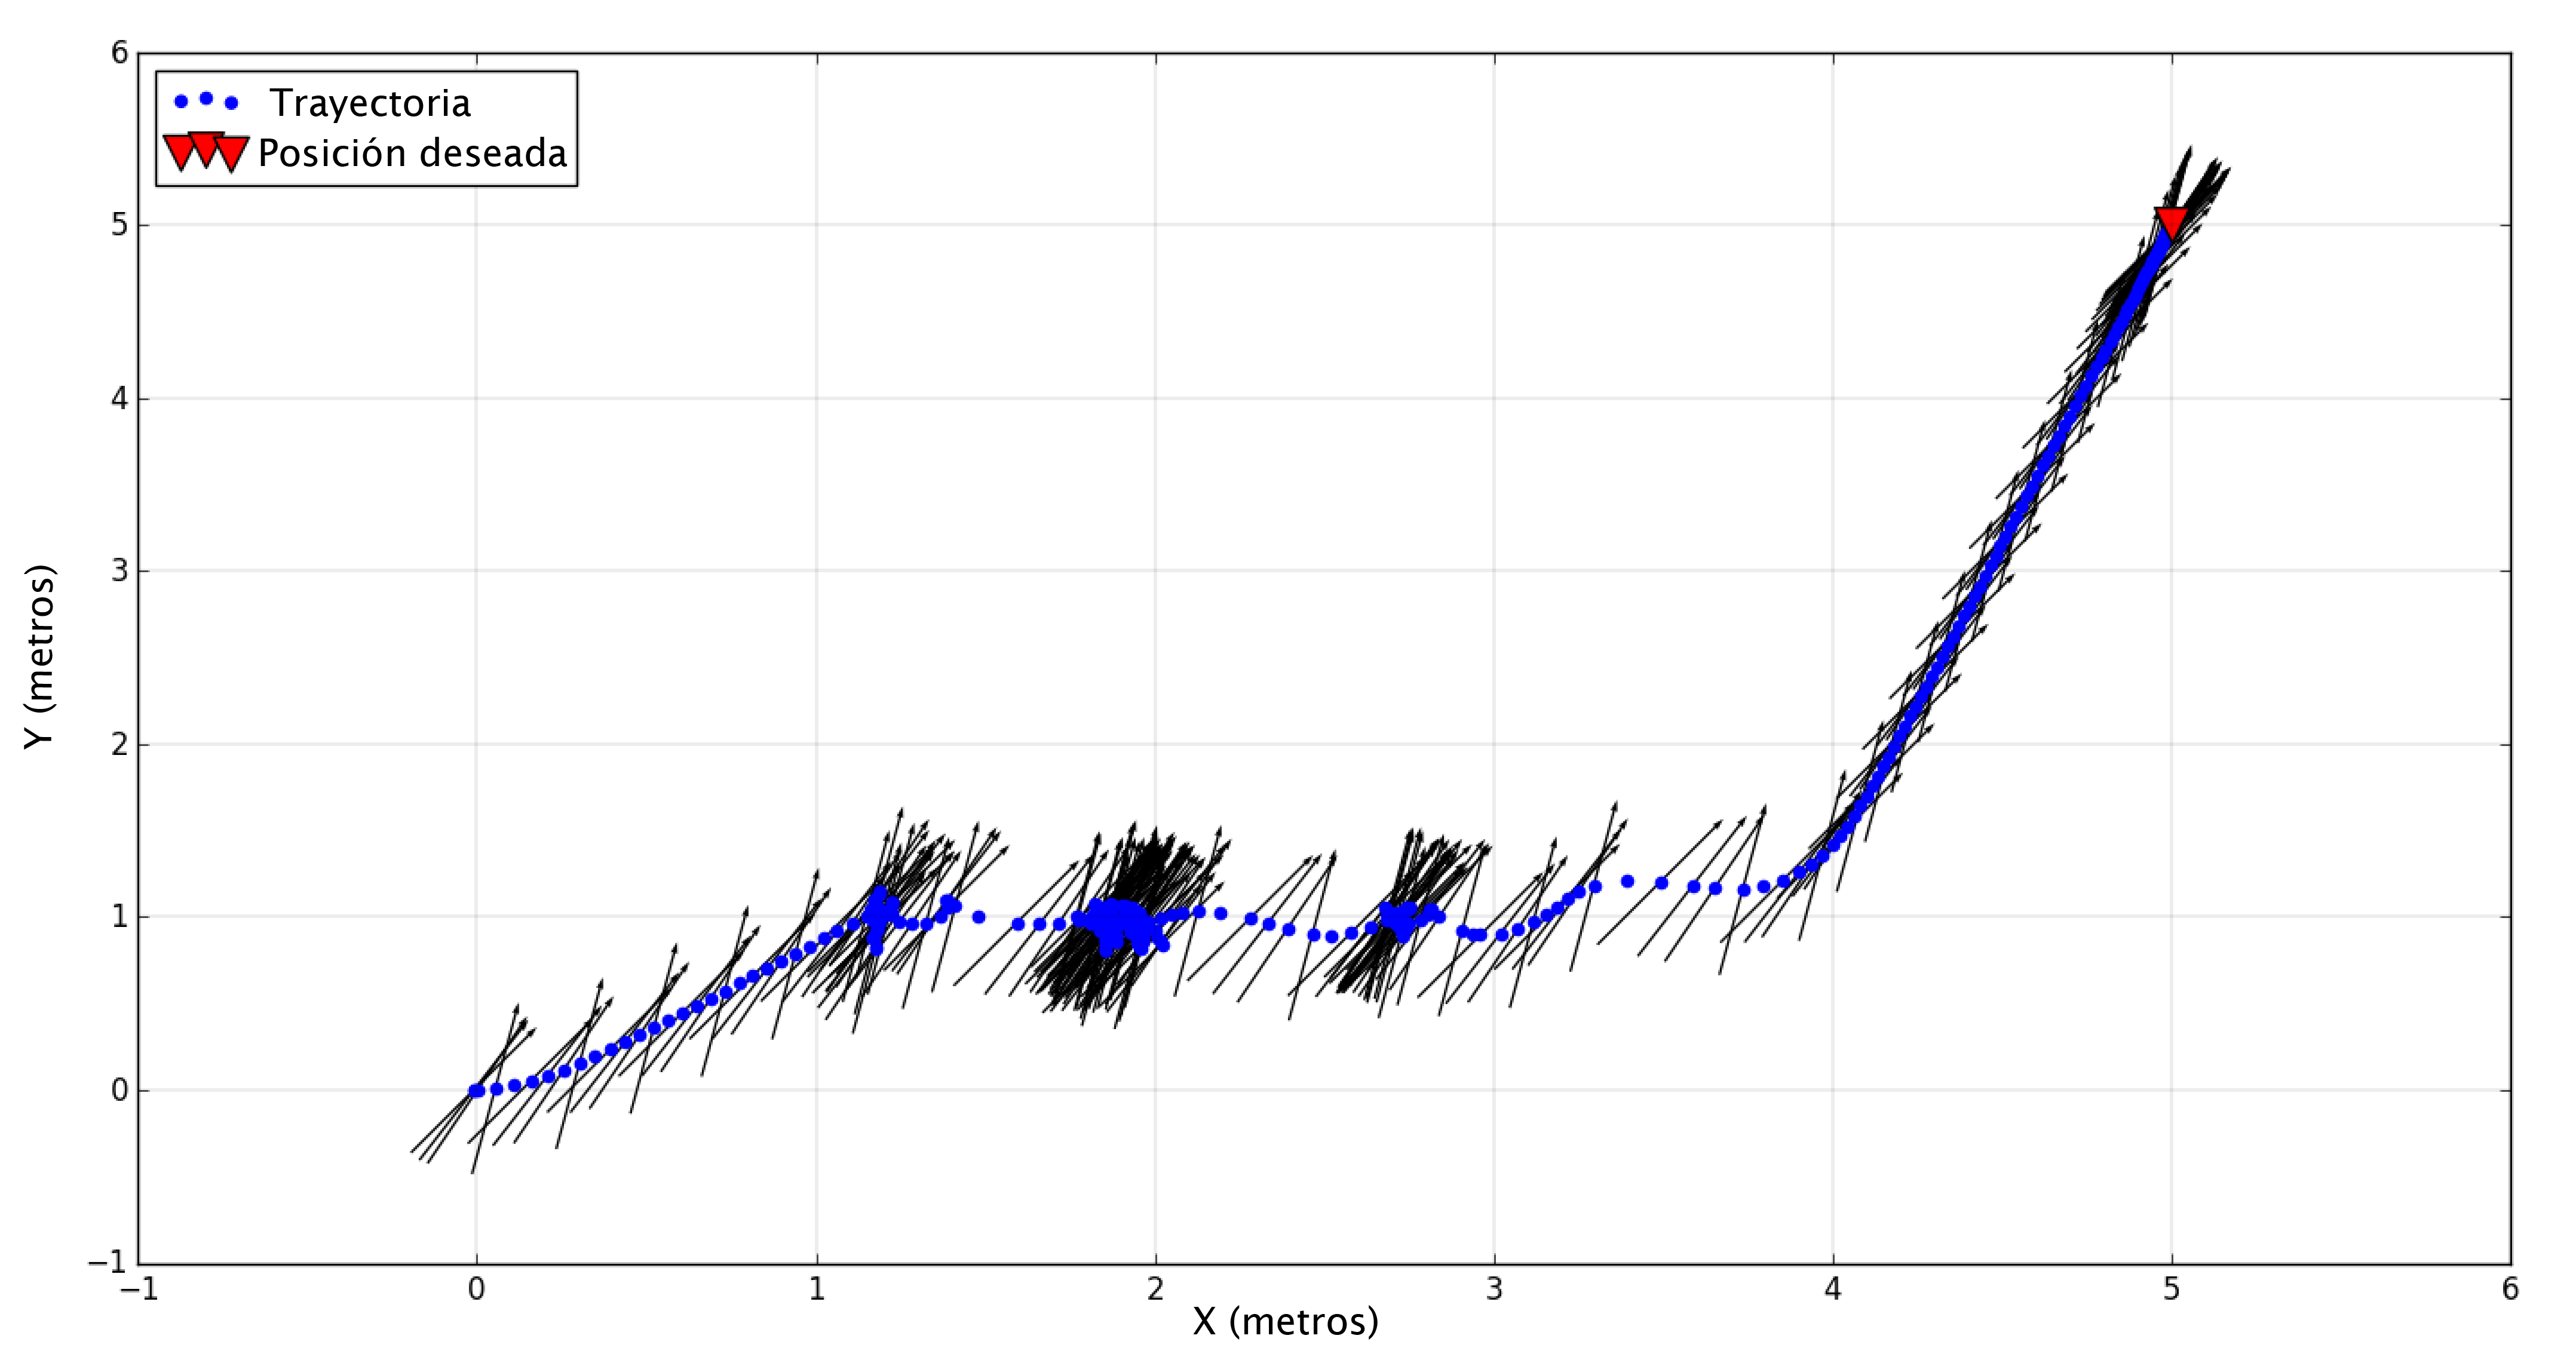
\includegraphics
        [width=.69\textwidth]{images/fattr_slam.png}}
        \subfigure[Fuerzas de repulsión aplicado al robot móvil en tiempo real]{\label{fig:etiquetaB}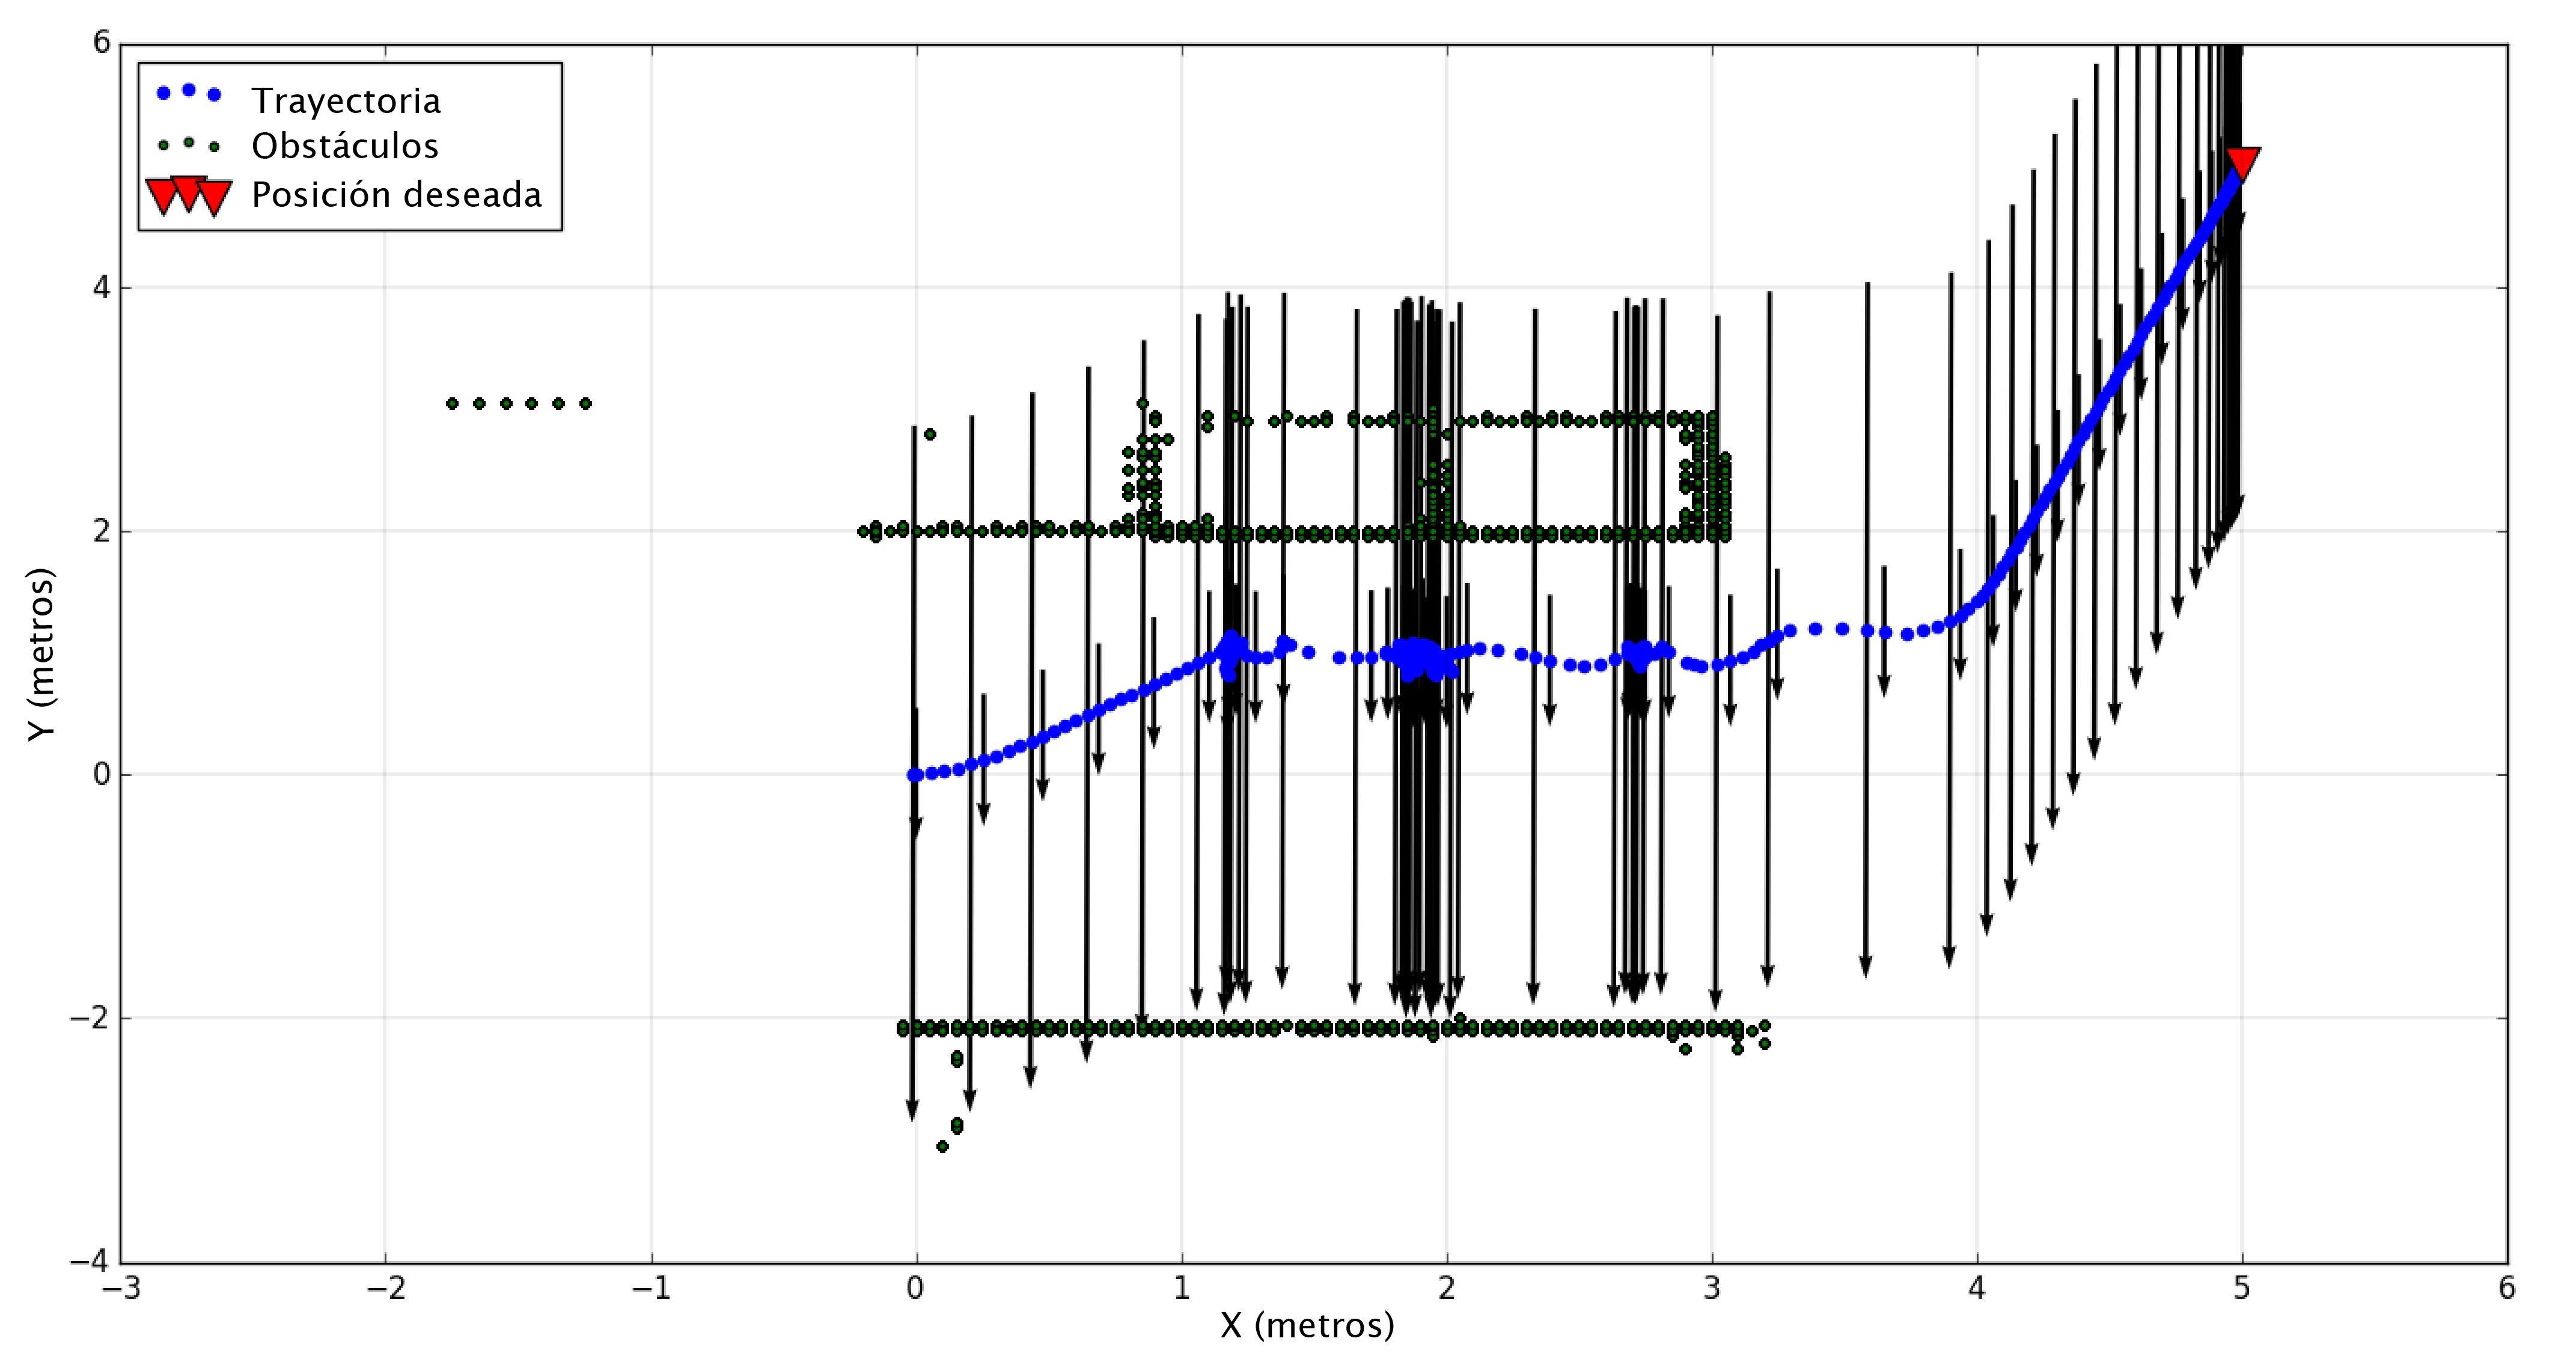
\includegraphics
        [width=.69\textwidth]{images/frep_slam.png}}
        \subfigure[Fuerzas de navegación aplicado al robot móvil en tiempo real]{\label{fig:etiquetaC}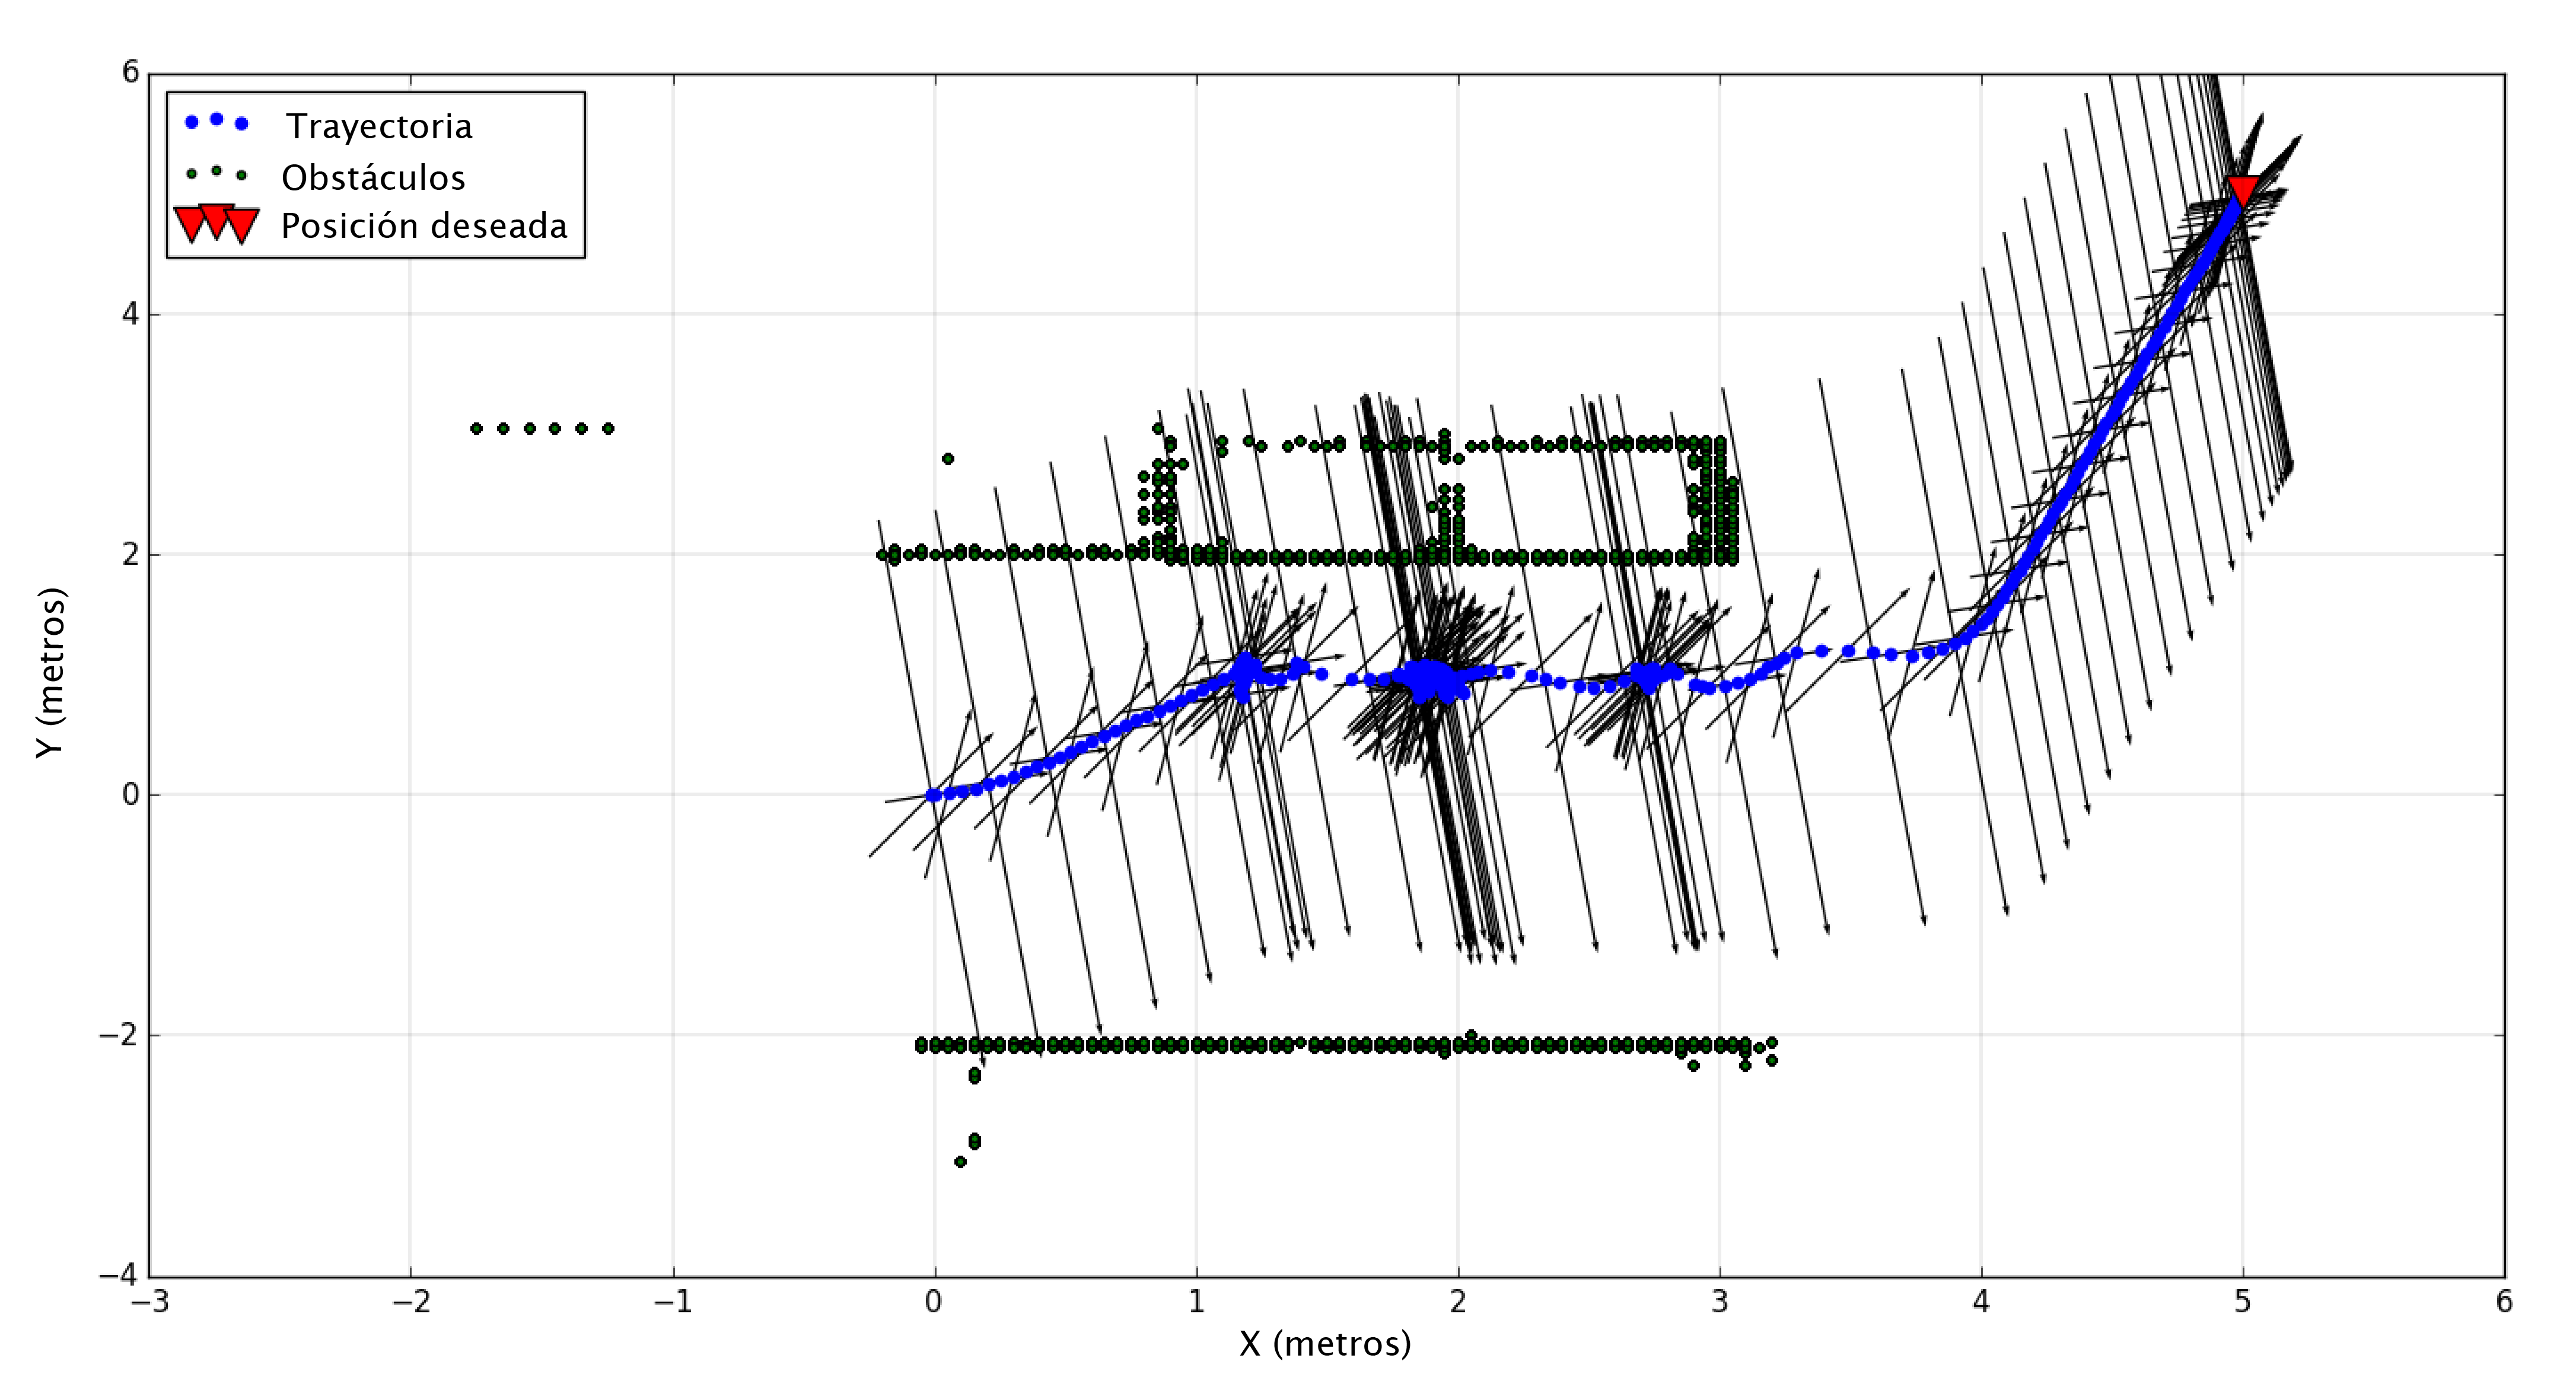
\includegraphics
        [width=.69\textwidth]{images/fnav_slam.png}}
    \end{center}
  \captionsetup{font=footnotesize}
    \caption{\label{fig:Kbki_slam}Campos atractivos y repulsivos, y la trayectoria que el robot real sigue 
    usando datos en línea provenientes del sensor lidar montado en la parte superior del Kobuki.}
\end{figure}

%\begin{figure}%[ht!]
%  \centering \footnotesize
%  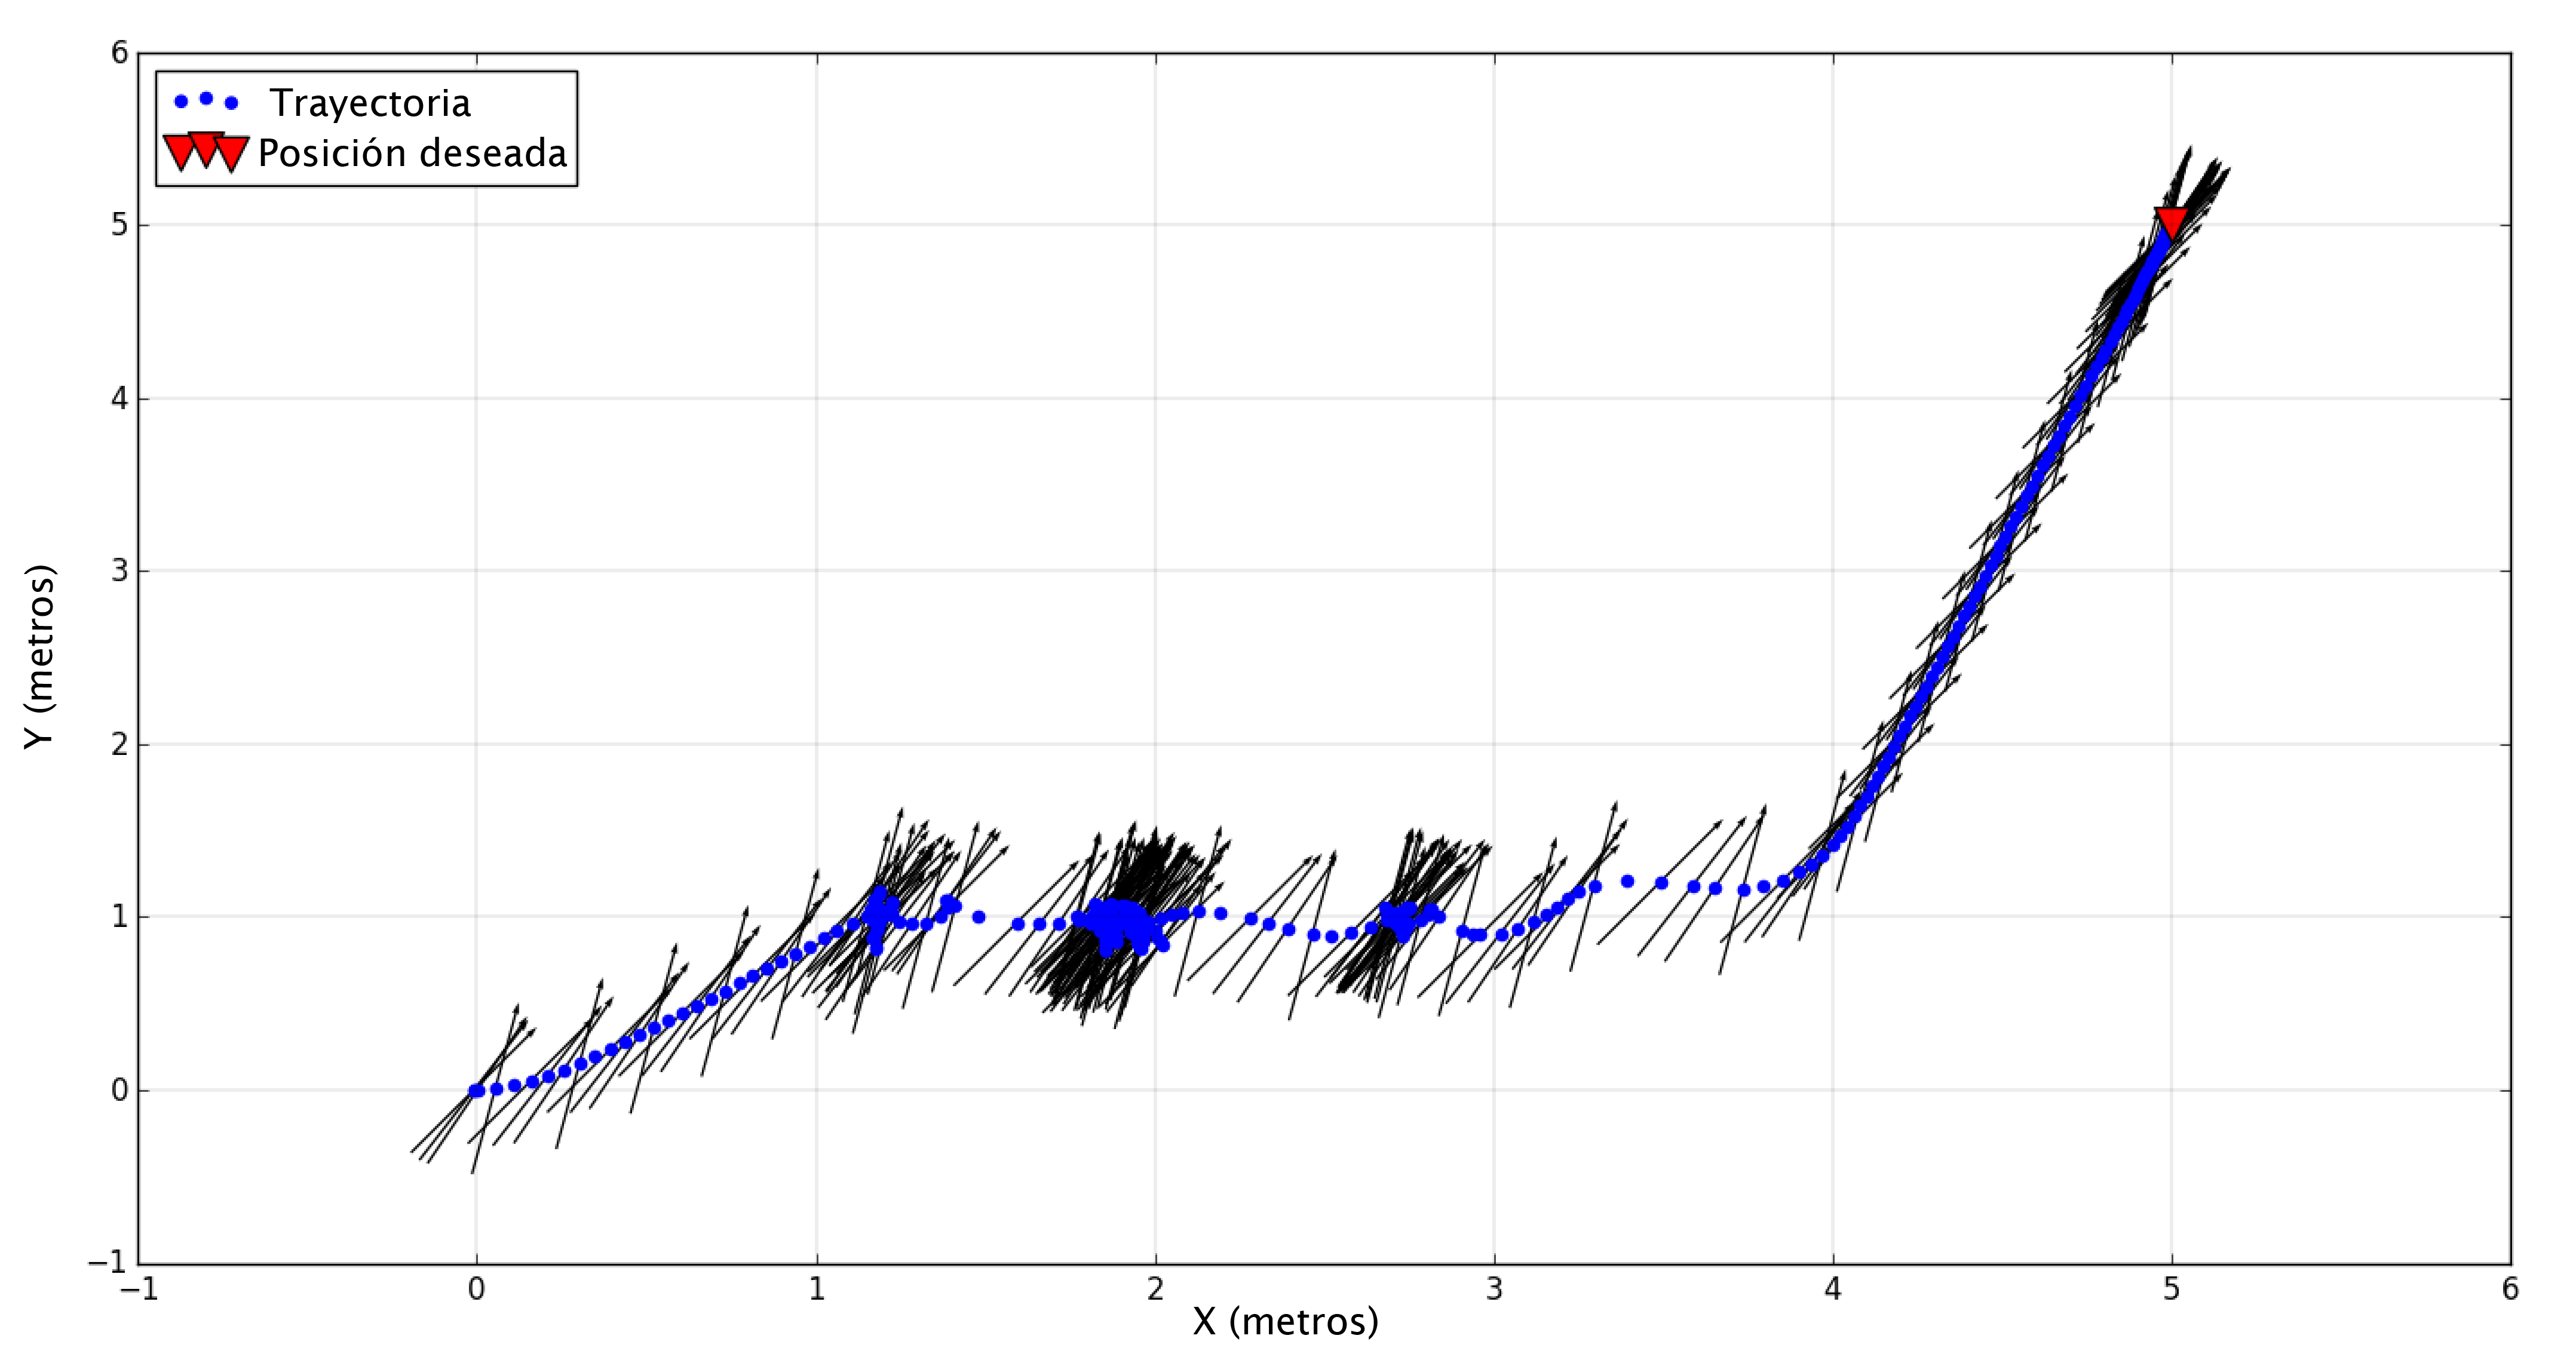
\includegraphics[width=0.80\textwidth]{images/fattr_slam.png}
%  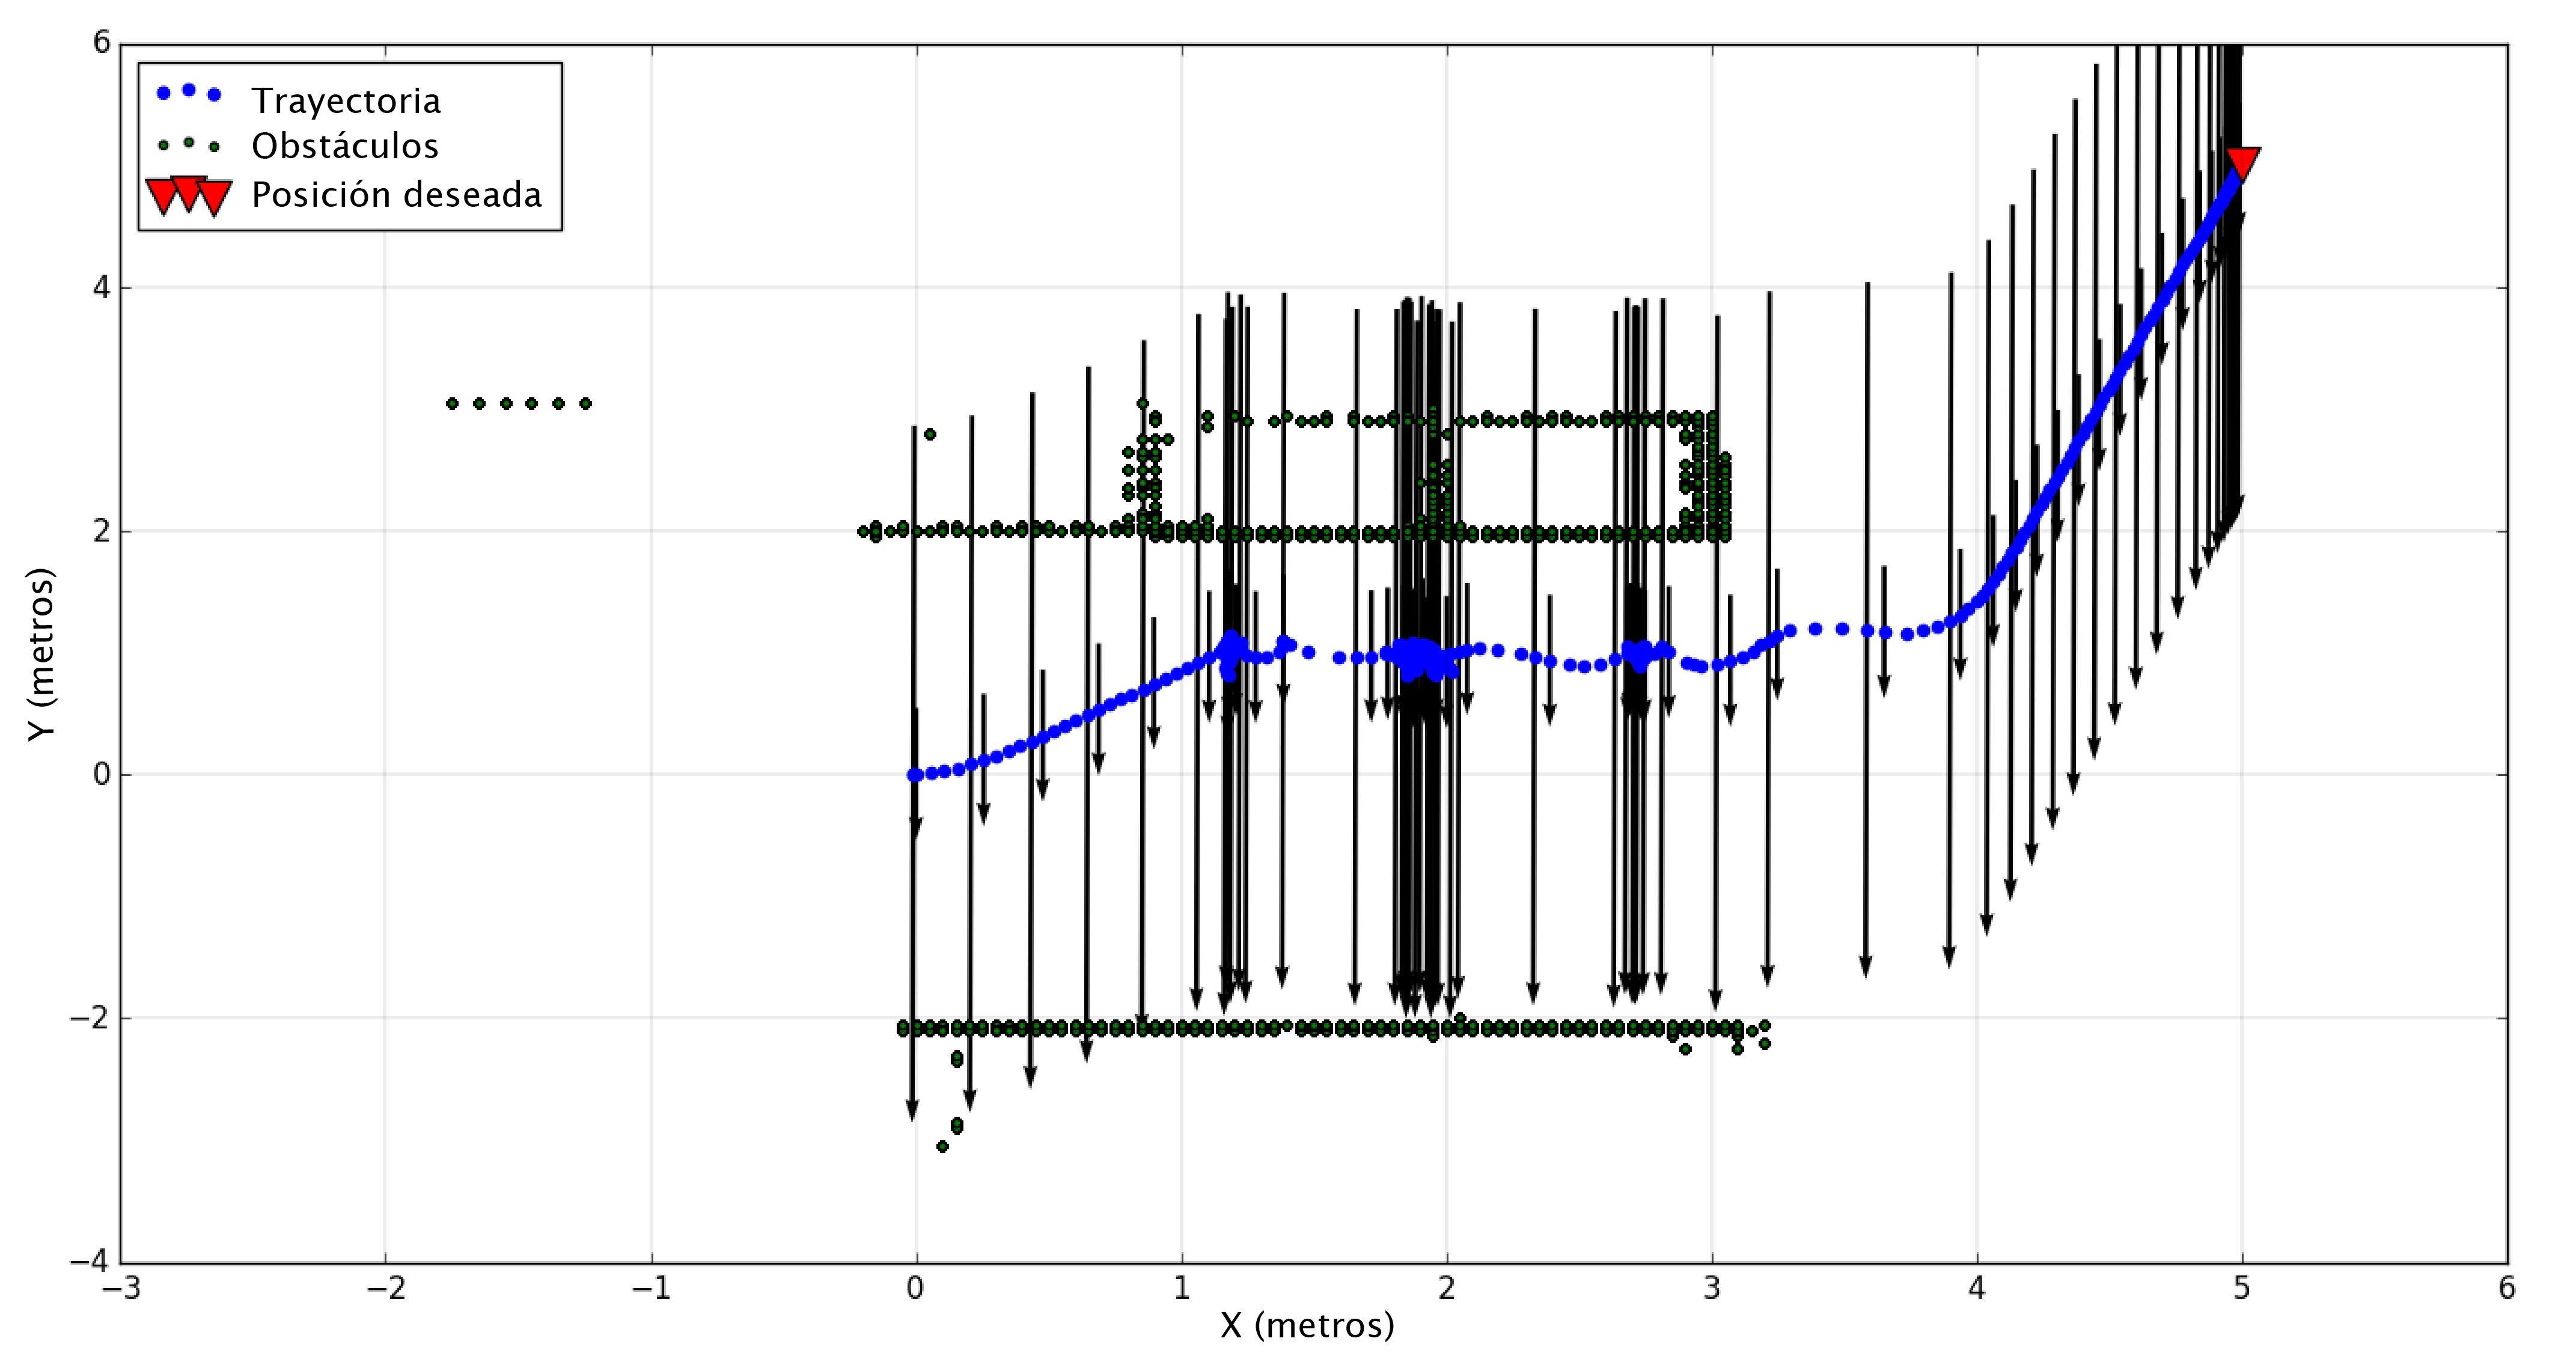
\includegraphics[width=0.80\textwidth]{images/frep_slam.png}
%  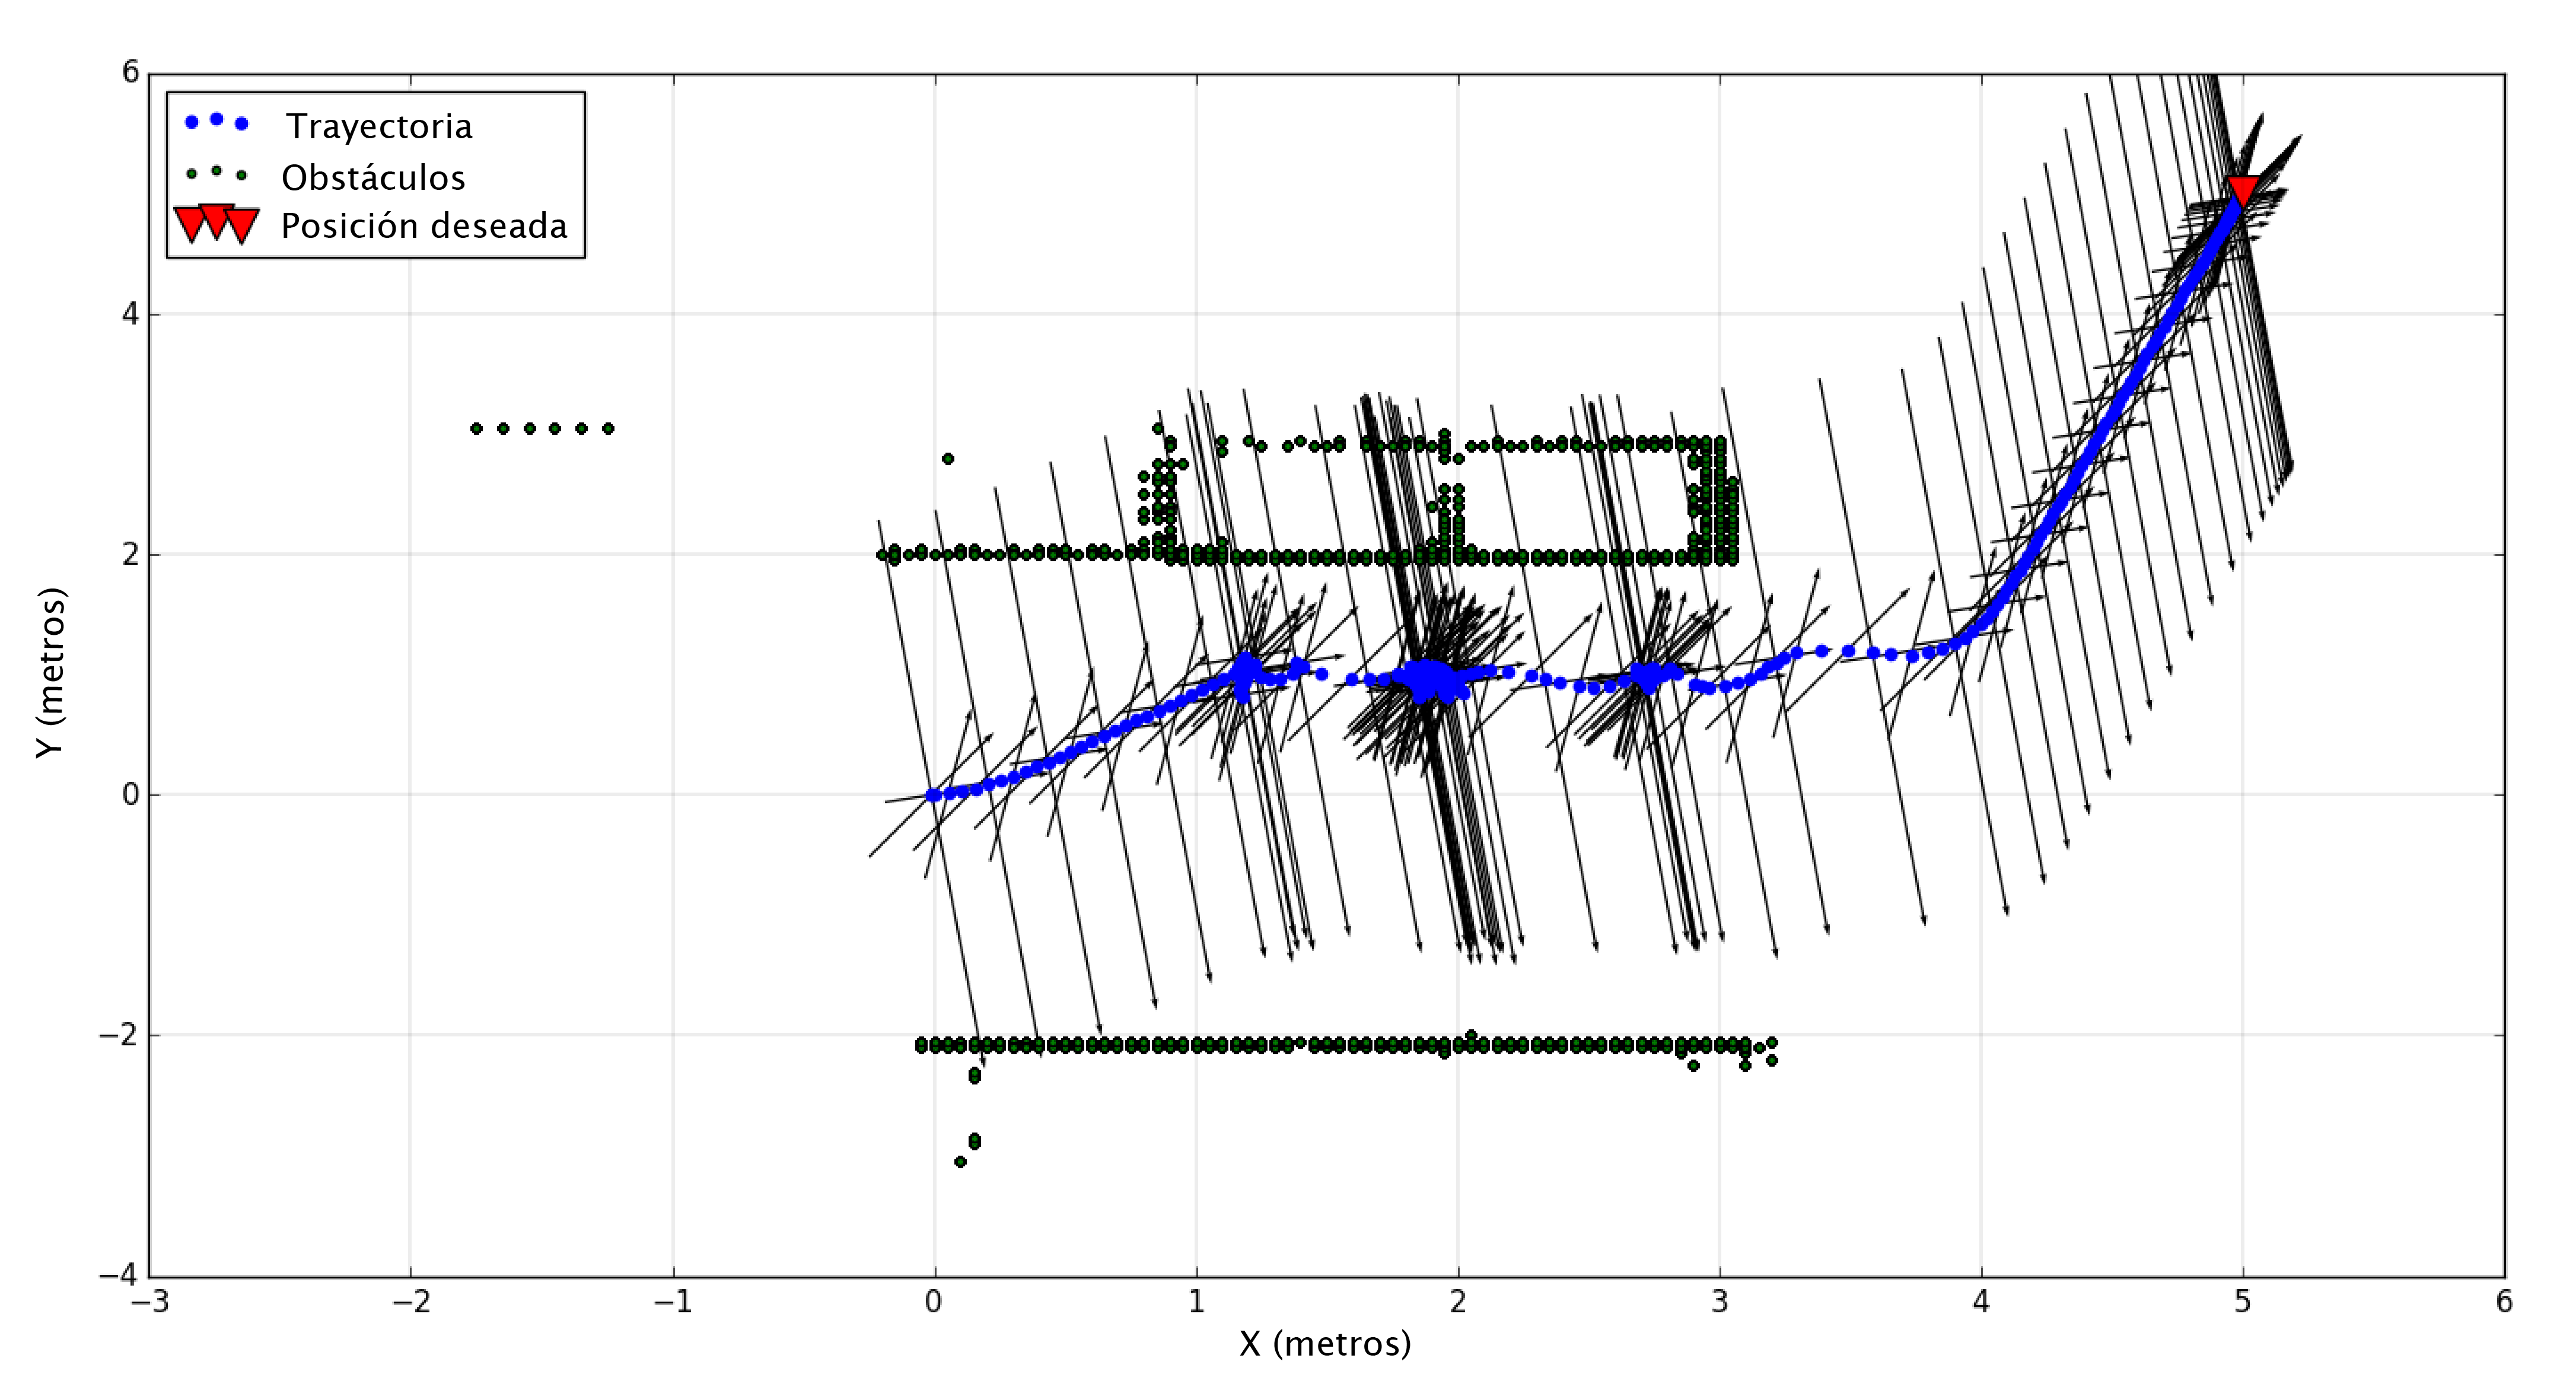
\includegraphics[width=0.80\textwidth]{images/fnav_slam.png}
%  \captionsetup{font=footnotesize}
%  \caption{Campos atractivos y repulsivos, y la trayectoria que el robot real sigue 
%  usando datos en línea provenientes del sensor lidar montado en la parte superior del 
%  Kobuki.}
%  \label{fig:Kbki_slam}
%\end{figure}

Para el algoritmo SLAM se usó el paquete de códido abierto \textit{gmapping}. El paquete 
\textit{gmapping} permite crear un mapa en dos dimensiones a partir de los datos de sensor 
lidar y la odometría del robot móvil. Al momento de iniciar el paquete \textit{gmapping}, 
este crea tópicos a los cuales se debe enviar los datos de la odometría del robot y los datos 
del sensor lidar. Con la información dada el nodo de SLAM publica las dimensiones del mapa 
dentro de un tópico. Para que el Kobuki se mueva con respecto al mapa generado, el marco de 
referencia del Kobuki se toma como el marco de referencia del sensor lidar. El nodo de 
SLAM tiene un alcance máximo de mapeo de 8 metros, tiene un tamaño de mapa en píxeles de 
512 x 512 y una resolución de mapa de 2.5 centímetros por cada celda del mapa. Además el 
algoritmo muestrea la cantidad de mediciones que envía el lidar, por tal motivo el mapa 
obtenido es bastante uniforme y preciso con respecto a las posiciones de los obstáculos 
dentro del mapa. 

Para  realizar que el robot se pueda desplazar de forma autónoma dentro del ambiente,se 
obtiene las posiciones del mapa ($X_{M}, Y_{M}$), los cuales son enviados al algoritmo 
de campos potenciales como obstáculos para que el robot pueda generar su propia 
trayectoria. Para realizar esta prueba se elige una posición deseado en el mapa. La 
posición deseada es $(x = 5, y = 5)$. En la figura \ref{fig:Kbki_slam} (a) se muestra 
la trayectoria del robot (puntos azules) que se va desplazando hacia la posición 
deseada. Además se puede ver que las flechas de color negro tienen una dirección, esto
indica la orientación necesaria que debe tener el robot para que llegue hacia la meta, 
asimismo el tamaño de las flechas indican la velocidad a la que debe ir el robot para 
que llegue al punto deseado. 

En la figura \ref{fig:Kbki_slam} (b) se muestra los obstáculos (puntos verdes), se 
aprecia con mayor claridad y uniformidad las posiciones de los obstáculos. Esto se debe 
a que el algoritmo muestrea la cantidad de mediciones que hace el sensor lidar y añade 
la odometría del robot, permitiendo estimar con mayor precisión las posiciones de los 
obstáculos. También se puede observar las flechas de color negro que tienen una dirección 
hacia afuera de los obstaćulos. La dirección de las flechas es según la trayectoria 
(puntos azules) del robot, en este caso el robot se acerca hacia los obstáculos que se 
encuentran en los valores del eje $Y$ positivo y el algoritmo de campos potenciales 
genera fuerzas de repulsión para que el robot evite los obstáculos. Se muestra una 
acumulación de puntos en diferentes partes de la trayectoria, y a su vez se nota una 
mayor concentración de fuerzas de repulsión en dichas partes, esto se debe a la interacción 
del movimiento del robot para no chocarse con los obstáculos y generar una nueva trayectoria 
hacia el punto deseado. Finalmente, en la figura \ref{fig:Kbki_slam} (c) se muestra las sumas 
de las fuerzas de atracción y las fuerzas de repulsión que hacen que el robot pueda ir a la 
posición deseada y a su vez evite los obstáculos del lugar.

\begin{figure}
  \centering \footnotesize
  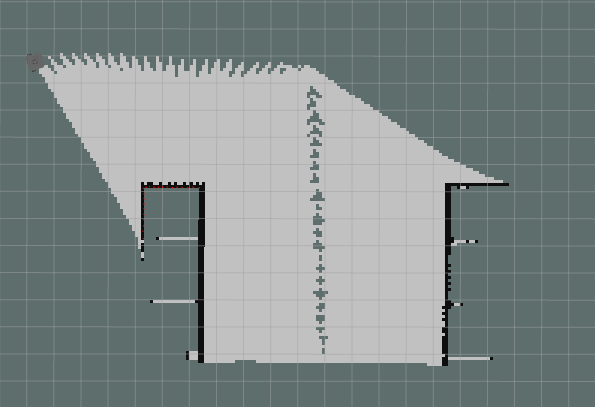
\includegraphics[width=0.80\textwidth]{images/map_slam.png}
  \captionsetup{font=footnotesize}
  \caption{Mapa en dos dimensiones - SLAM}
  \label{fig:SLAM_2D}
\end{figure}

La figura \ref{fig:SLAM_2D} muestra el mapa generado por el paquete \textit{gmapping}. Como 
se puede ver en la imagen, el mapa esta compuesto por tres colores diferentes. Cada color 
de la imagen tiene un significado. El color verdoso significa un lugar desconocido, esto 
quiere decir los lugares por donde el robot móvil no ha explorado o navegado. El color 
plomo claro, significa un lugar conocido, esto quiere decir el lugar por donde el robot 
móvil o el sensor lidar ha recorrido. Finalmente, el color negro este color representa a 
los obstáculos mapeado dentro del entorno explorado. Este mapa ayuda a que el robot pueda 
reconocer con exactitud los lugares que ha explorado, los obstáculos y los lugares que aún 
le falta por recorrer.

\section{Resultado del mapa en tres dimensiones}
En esta sección se explicará las pruebas que se realizaron para poder validar el mapa en 
tres dimensiones con el sistema mecánico propuesto. Se realizarón pruebas de validación 
del algoritmo para la construcción del mapa en 3D dentro de una caja cerrada y dentro de 
un pasadizo cerrado. Las pruebas consistieron en dejar el sistema mecánico de manera 
estática y empezar a realizar mediciones mientras el lidar giraba en 360\grad~ y el 
servomotor rotaba en un ángulo de abertura de $\pm$ 15\grad~.

\subsection{Mapa en tres dimensiones de una caja}
\label{sec:MapaCaja}
\begin{figure}
  \centering \footnotesize
  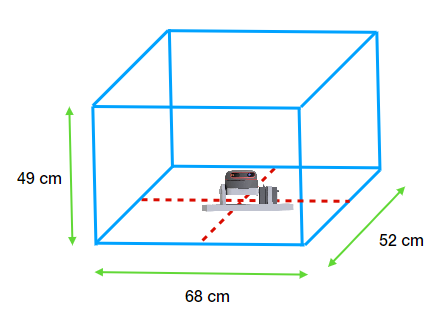
\includegraphics[width=0.70\textwidth]{images/caja_lidar3D.png}
  \captionsetup{font=footnotesize}
  \caption{Dimensiones de la caja real donde se realizó las pruebas.}
  \label{fig:dim_cajaReal}
\end{figure}

Para realizar la primera prueba, se utilizó una caja real en el cual fue colocado 
el sistema mecánico del sensor lidar para realizar las mediciones. En la figura 
\ref{fig:dim_cajaReal} se muestra las dimensiones de la caja donde se hizo las 
pruebas. Como primer paso se coloco el sistema mecánico en el centro de la caja, esto
ayuda a conocer las posiciones de las paredes de la caja en el plano cartesiano. Una 
vez colocado el sensor, fue dejado por 40 segundos para que realicé las mediciones del 
ambiente. El sensor lidar y el servomotor fueron controlados a través de un Raspberry 
Pi3. La información enviada por el sensor y el servomotor son recibidos por el Raspberry 
Pi3, el cual se encarga de enviar los datos de forma remota hacia una computadora. Estos 
datos son almacenados para ser procesadas posteriormente.

\begin{figure}[ht!]
     \begin{center}
        \subfigure[]{\label{fig:etiquetaA}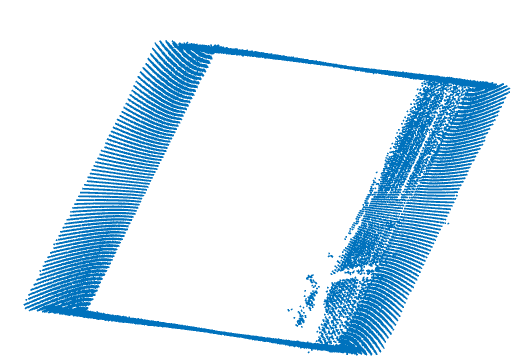
\includegraphics[width=.32\textwidth]{images/caja3D_1.png}}
        \subfigure[]{\label{fig:etiquetaB}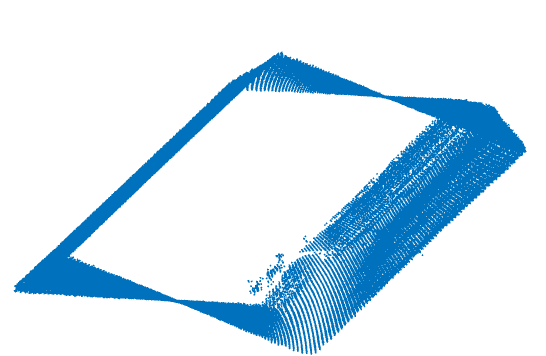
\includegraphics[width=.32\textwidth]{images/caja3D_2.png}}
        \subfigure[]{\label{fig:etiquetaC}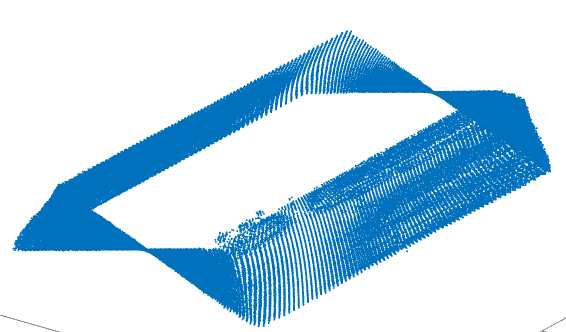
\includegraphics[width=.32\textwidth]{images/caja3D_3.png}}
        \subfigure[]{\label{fig:etiquetaC}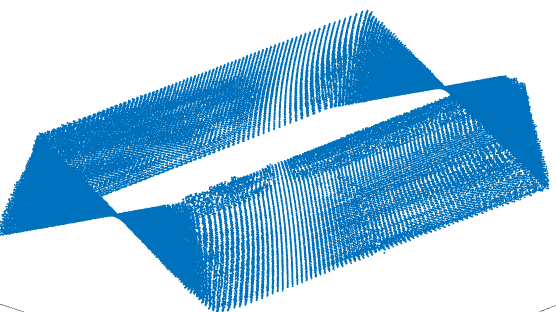
\includegraphics[width=.32\textwidth]{images/caja3D_4.png}}
        \subfigure[]{\label{fig:etiquetaC}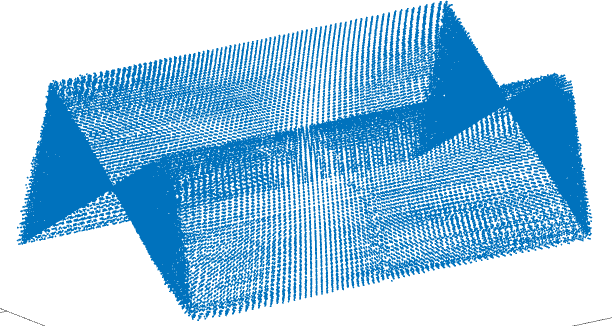
\includegraphics[width=.32\textwidth]{images/caja3D_5.png}}
        \subfigure[]{\label{fig:etiquetaC}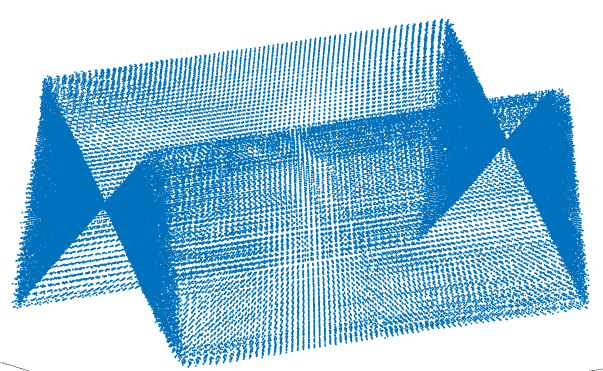
\includegraphics[width=.32\textwidth]{images/caja3D_6.png}}
        \subfigure[]{\label{fig:etiquetaC}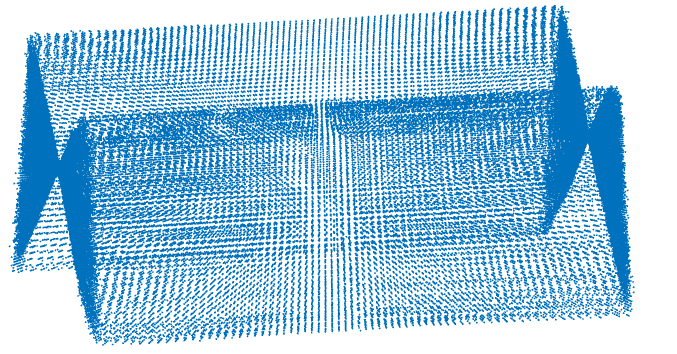
\includegraphics[width=.32\textwidth]{images/caja3D_7.png}}
        \subfigure[]{\label{fig:etiquetaC}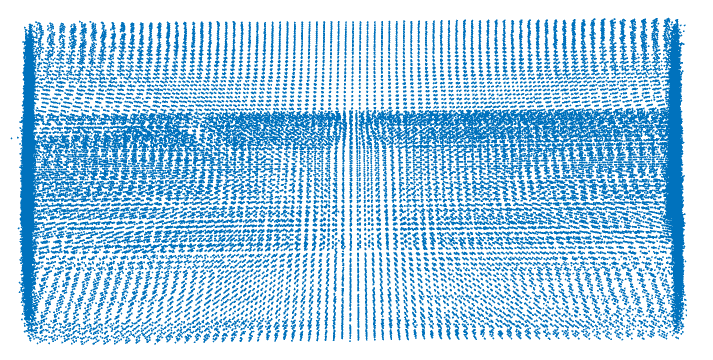
\includegraphics[width=.32\textwidth]{images/caja3D_8.png}}
        \subfigure[]{\label{fig:etiquetaC}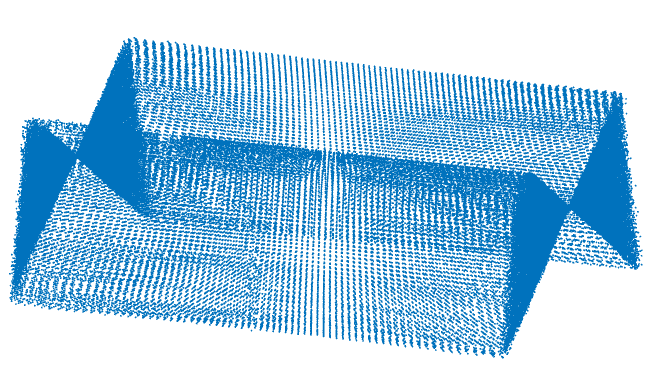
\includegraphics[width=.32\textwidth]{images/caja3D_9.png}}
    \end{center}
  \captionsetup{font=footnotesize}
    \caption{\label{fig:Caja3D}Mapa en tres dimensiones de una caja. El crecimiento del mapa tridimensional 
    va en sentido horario.}
\end{figure}

%\begin{figure}
%  \centering \footnotesize
%  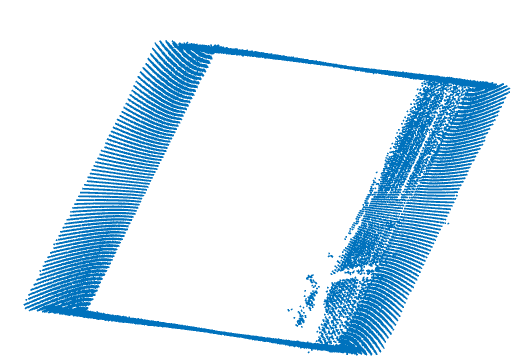
\includegraphics[width=0.40\textwidth]{images/caja3D_1.png}
%  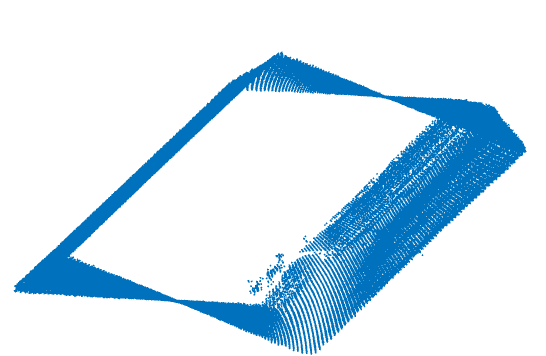
\includegraphics[width=0.40\textwidth]{images/caja3D_2.png}
%  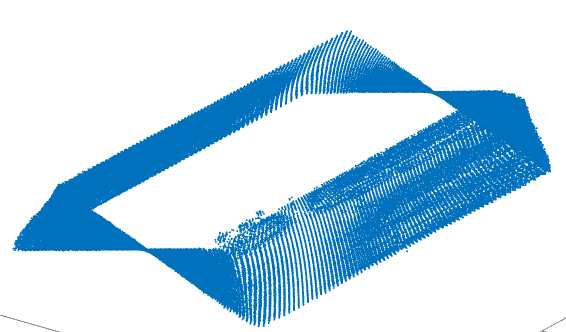
\includegraphics[width=0.40\textwidth]{images/caja3D_3.png}
%  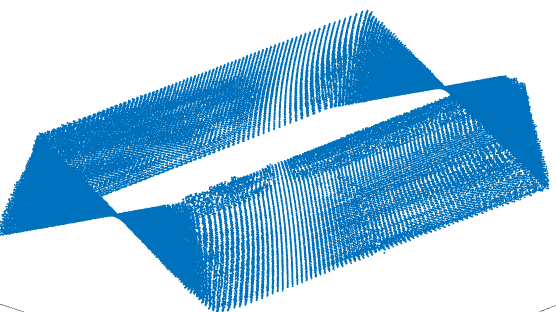
\includegraphics[width=0.40\textwidth]{images/caja3D_4.png}
%  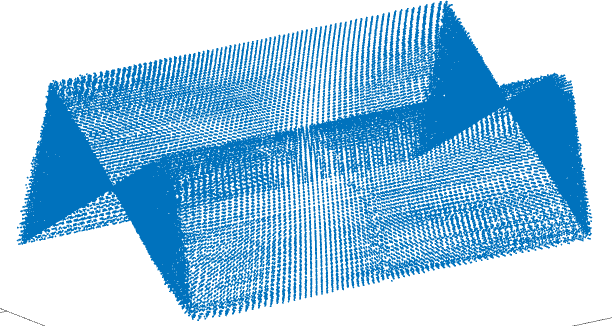
\includegraphics[width=0.40\textwidth]{images/caja3D_5.png}
%  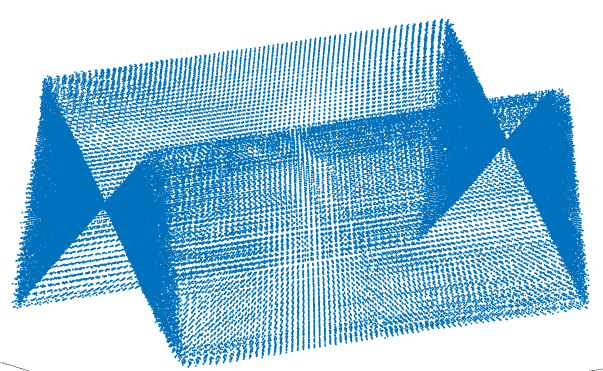
\includegraphics[width=0.40\textwidth]{images/caja3D_6.png}
%  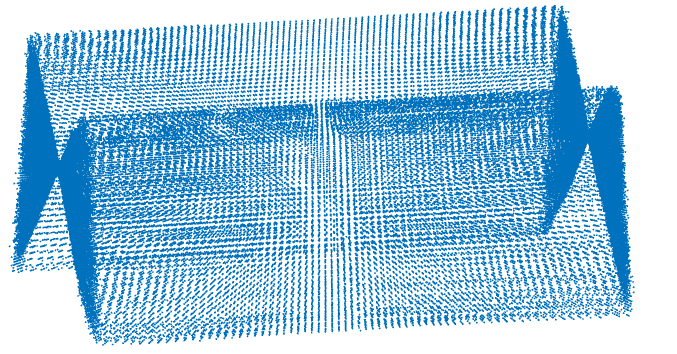
\includegraphics[width=0.40\textwidth]{images/caja3D_7.png}
%  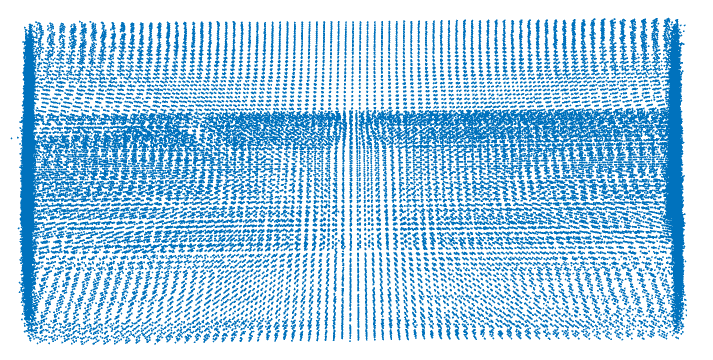
\includegraphics[width=0.40\textwidth]{images/caja3D_8.png}
%  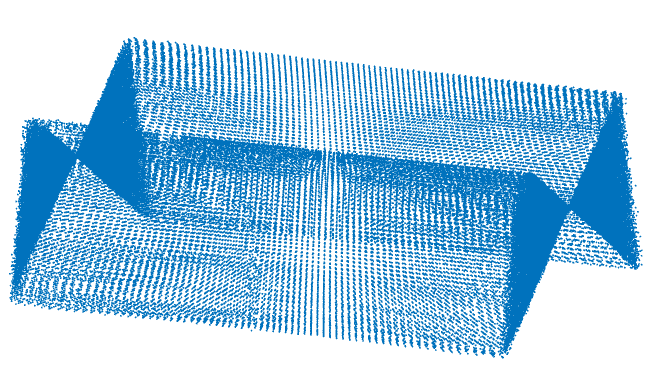
\includegraphics[width=0.50\textwidth]{images/caja3D_9.png}
%  \captionsetup{font=footnotesize}
%  \caption{Mapa en tres dimensiones de una caja. El crecimiento del mapa tridimensional 
%  de la caja va en sentido horario.}
%  \label{fig:Caja3D}
%\end{figure}

En las anteriores secciones se mencionó el proceso para la construcción del mapa en 
tres dimensiones con los datos del sensor lidar y del servomotor. En la figura 
\ref{fig:Caja3D} se muestran los resultados obtenidos. El crecimiento de la caja va en
aumento de izquierda a derecha donde se puede apreciar las paredes de la caja y la forma
de rectángulo que tiene. De la figura \ref{fig:Caja3D} se puede notar que dos paredes de 
la caja tienen forma de dos triángulos unidos por un vértice, esto es debido al movimiento 
de traslación del sistema mecánico. En el capítulo anterior se explico sobre le movimiento 
de rotación y traslación que tiene el sistema mecánico (figura \ref{f:Rot3D} (b)) para la 
construcción del mapa tridimensional. El servomotor genera un movimiento de traslación al 
sensor lidar, por tal motivo hace que el lidar tenga puntos ciegos al momento de rotar 
sobre el ángulo de abertura ($\pm$ 15\grad~) que forma el eje del servomotor. Asimismo,
se puede observar que existe una pequeña inclinación en las paredes del modelo 
tridimensional generado pero sin mucha consideración.

\begin{figure}
  \centering \footnotesize
  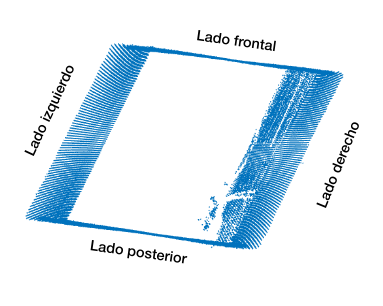
\includegraphics[width=0.60\textwidth]{images/lados_caja.png}
  \captionsetup{font=footnotesize}
  \caption{Nombre de las paredes de la caja.}
  \label{fig:paredCaja}
\end{figure}

\begin{figure}[ht!]
     \begin{center}
        \subfigure[Distribución normal del lado izquierdo de la caja real]{\label{fig:hist_Izq}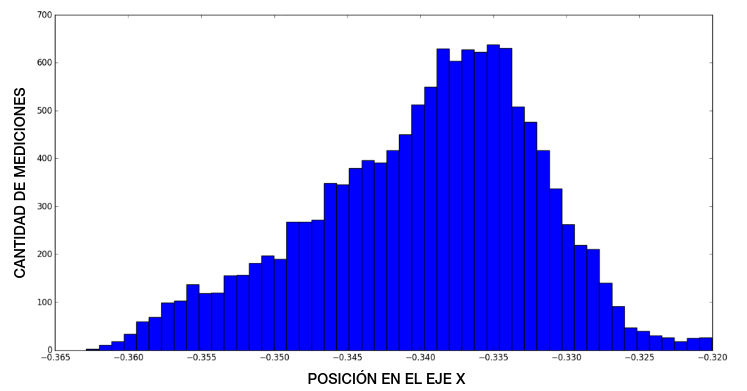
\includegraphics
        [width=.75\textwidth]{images/hist_izquierda_caja.png}}
        \subfigure[Distribución normal del lado derecho de la caja real]{\label{fig:hist_Dere}\includegraphics
        [width=.75\textwidth]{images/hist_derecha_caja.png}}
    \end{center}
  \captionsetup{font=footnotesize}
    \caption{\label{}Distribución de las mediciones con respecto a la posición (x) de las 
    paredes derecha e izquierda de la caja real.}
\end{figure}

%\begin{figure}
%  \centering \footnotesize
%  \includegraphics[width=0.90\textwidth]{images/hist_izquierda_caja.png}
%  \captionsetup{font=footnotesize}
%  \caption{Distribución normal del lado izquierdo de la caja real.}
%  \label{fig:hist_Izq}
%\end{figure}

%\begin{figure}
%  \centering \footnotesize
%  \includegraphics[width=0.90\textwidth]{images/hist_derecha_caja.png}
%  \captionsetup{font=footnotesize}
%  \caption{Histograma del lado derecho de la caja real.}
%  \label{fig:hist_Dere}
%\end{figure}

Después de haber obtenido el modelo en tres dimensiones, de la caja real, se midió 
el error en la posición las paredes de la caja con respecto a la posición de la nube 
de puntos obtenido. Para hacer esto se colocó un nombre a cada pared, como se muestra en 
la figura \ref{fig:paredCaja}, para poder diferenciar cada lado. Como se mencionó 
anteriormente, para realizar esta prueba el sistema mecánico tuvo que ser colocado en 
el centro de la caja. El lado izquierdo de la caja tiene una posición de ($X_{c} = 
-0.34$), ya que el largo de la caja es de 68 cm (figura \ref{fig:dim_cajaReal}). En 
la figura \ref{fig:hist_Izq} se muestra el histograma del lado izquierdo de la caja, 
donde se aprecia una distribución normal. Las barras dentro de la gráfica significa la
cantidad de mediciones con respecto a las posiciones en el eje de la caja ($X_{c}$). De los 
datos obtenidos de la nube de puntos, del lado izquierdo de la caja, se obtuvo un 
promedio $\bar{u} = -0.339$ y una desviación estándar de $\sigma = 0.007$. El lado 
derecho de la caja tiene una posición de $(X_{c} = 0.34)$; en la figura \ref{fig:hist_Dere} 
se muestra una distribución normal con una concentración de mediciones en la posición del 
lado derecho. Asimismo,se tiene un promedio $\bar{u} = 0.338$ y una desviación estándar 
de $\sigma = 0.011$.  

\begin{figure}[ht!]
     \begin{center}
        \subfigure[Distribución normal del lado frontal de la caja real]{\label{fig:hist_Front}\includegraphics
        [width=.60\textwidth]{images/hist_frontal_caja.png}}
        \subfigure[Distribución normal del lado posterior de la caja real]{\label{fig:hist_Post}\includegraphics
        [width=.60\textwidth]{images/hist_posterior_caja.png}}
    \end{center}
  \captionsetup{font=footnotesize}
    \caption{\label{}Distribución de las mediciones con respecto a la posición (y) de las 
    paredes frontal y posterior de la caja real.}
\end{figure}

%\begin{figure}
%  \centering \footnotesize
%  \includegraphics[width=0.80\textwidth]{images/hist_frontal_caja.png}
%  \captionsetup{font=footnotesize}
%  \caption{Histograma de la parte frontal de la caja real.}
%  \label{fig:hist_Front}
%\end{figure}

%\begin{figure}
%  \centering \footnotesize
%  \includegraphics[width=0.80\textwidth]{images/hist_posterior_caja.png}
%  \captionsetup{font=footnotesize}
%  \caption{Histograma de la parte posterior de la caja real.}
%  \label{fig:hist_Post}
%\end{figure}

Para el lado frontal y el lado posterior, también se realizó la medición del error de la
posición de la caja con respecto a la posición de la nube de puntos. El lado frontal de la
caja tiene una posición de $(Y_{c} = 0.26)$, ya que el ancho de la caja tiene una longitud
de 52 cm (figura \ref{fig:dim_cajaReal}). En la figura \ref{fig:hist_Front} se muestra una 
distribución normal con la mayor concentración de mediciones en los valores muy cercanos al 
0.26 en la posición en el eje de la caja $(Y_{c})$. Asimismo, se obtuvo un promedio de $\bar{u} 
= 0.256$ y una desviación estándar de $\sigma = 0.006$. El lado posterior de la caja tiene 
una posición de $(Y_{c} = -0.26)$; en la figura \ref{fig:hist_Post} se muestra una distribución
normal con la mayor cantidad de mediciones cerca al valor de -0.26. Se obtuvo un promedio de 
$\bar{u} = -0.26$ y una desviación estándar de $\sigma = 0.007$.

\subsection{Mapa en tres dimensiones de un pasadizo}
\begin{figure}
  \centering \footnotesize
  \includegraphics[width=0.80\textwidth]{images/esan_lidar.PNG}
  \captionsetup{font=footnotesize}
  \caption{Pasadizo de un centro de estudio}
  \label{fig:pasadizoEsan}
\end{figure}

Se realizo la segunda prueba dentro de un pasadizo, como se muestra en la figura 
\ref{fig:pasadizoEsan}. En esta figura se resalta la zona donde se realizó las pruebas 
con unas líneas rojas.Para esta prueba se coloco el sistema mecánico en el medio del 
rectángulo que forman las columnas del pasadizo, una vez colocado el sensor lidar con 
el servomotor se empezó a realizar las mediciones dentro del entorno por 70 segundos. Los 
datos del motor y del sensor fueron almacenados de forma remota en una computadora. 

Los resultados obtenidos del mapa tridimensional se muestra en la figura \ref{fig:pasadizo3D}, 
donde el crecimiento del mapa va en sentido horario. Las figuras muestran las paredes y las 
columnas del pasadizo, debido a que el sensor lidar tiene un alcance máximo de 8 metros la 
figura muestra otras zonas del pasadizo fuera de la sección mostrada en la figura 
\ref{fig:pasadizoEsan}. La estructura del pasadizo tiene una simetría con respecto a las 
paredes, ya que se puede ver que las columnas están posicionadas en el mismo lugar en 
ambos lados. Esto también se puede apreciar en el mapa 3D del pasadizo. En la nube de puntos 
obtenido en la prueba anterior, se notó una pequeña inclinación en las paredes de la caja 
pero en el caso de esta nube de puntos se nota las paredes bastante rectas sin ninguna 
inclinación. Esto es debido al rango mínimo permitido que tiene el sensor lidar (15 cm), 
el sensor lidar al mapear un lugar con dimensiones más grandes obtiene un mejor resultado en 
sus mediciones.

\begin{figure}[ht!]
     \begin{center}
        \subfigure[]{\label{fig:etiquetaA}\includegraphics[width=.47\textwidth]{images/pasadizo_8.png}}
        \subfigure[]{\label{fig:etiquetaB}\includegraphics[width=.47\textwidth]{images/pasadizo_7.png}}
        \subfigure[]{\label{fig:etiquetaC}\includegraphics[width=.47\textwidth]{images/pasadizo_6.png}}
        \subfigure[]{\label{fig:etiquetaC}\includegraphics[width=.47\textwidth]{images/pasadizo_5.png}}
        \subfigure[]{\label{fig:etiquetaC}\includegraphics[width=.47\textwidth]{images/pasadizo_4.png}}
        \subfigure[]{\label{fig:etiquetaC}\includegraphics[width=.47\textwidth]{images/pasadizo_3.png}}
        \subfigure[]{\label{fig:etiquetaC}\includegraphics[width=.47\textwidth]{images/pasadizo_2.png}}
        \subfigure[]{\label{fig:etiquetaC}\includegraphics[width=.47\textwidth]{images/pasadizo_1.png}}
    \end{center}
  \captionsetup{font=footnotesize}
    \caption{\label{fig:pasadizo3D}Mapa en tres dimensiones de un pasadizo. El crecimiento del mapa 
    tridimensional del pasadizo va en sentido horario.}
\end{figure}

%\begin{figure}
%  \centering \footnotesize
%  \includegraphics[width=0.49\textwidth]{images/pasadizo_8.png}
%  \includegraphics[width=0.49\textwidth]{images/pasadizo_7.png}
%  \includegraphics[width=0.49\textwidth]{images/pasadizo_6.png}
%  \includegraphics[width=0.49\textwidth]{images/pasadizo_5.png}
%  \includegraphics[width=0.49\textwidth]{images/pasadizo_4.png}
%  \includegraphics[width=0.49\textwidth]{images/pasadizo_3.png}
%  \includegraphics[width=0.49\textwidth]{images/pasadizo_2.png}
%  \includegraphics[width=0.49\textwidth]{images/pasadizo_1.png}
%  \captionsetup{font=footnotesize}
%  \caption{Mapa en tres dimensiones de un pasadizo. El crecimiento del mapa tridimensional 
%  pasadizo va en sentido horario.}
%  \label{fig:pasadizo3D}
%\end{figure}

\section{Resultado del mapa 3D mientras el robot se mueve}
\begin{figure}
  \centering \footnotesize
  \includegraphics[width=0.80\textwidth]{images/prueba_cajas.JPG}
  \captionsetup{font=footnotesize}
  \caption{Túnel construido por cajas de cartón, para probar el algoritmo
  de mapeo tridimensional mientras el robot se mueve.}
  \label{fig:tunel201}
\end{figure}
En esta sección se explica los resultados que se obtuvo al realizar el mapa en tres
dimensiones mientras el robot Kobuki se desplaza sobre un entorno. Para esta prueba se utilizó 
como prototipo de túnel dos cajas unidas, el cual se muestra en la figura \ref{fig:tunel201}. 
El túnel prototipo tiene 194 cm de largo, la entrada del túnel tiene un ancho de 69 cm y en la 
mitad de este tiene un ancho de 92 cm.

\begin{figure}[ht!]
     \begin{center}
        \subfigure[]{\label{fig:etiquetaB}\includegraphics[width=.22\textwidth]{images/3DMOV_2.png}}
        \subfigure[]{\label{fig:etiquetaC}\includegraphics[width=.45\textwidth]{images/3DMOV_3.png}}
        \subfigure[]{\label{fig:etiquetaC}\includegraphics[width=.45\textwidth]{images/3DMOV_6.png}}
        \subfigure[]{\label{fig:etiquetaC}\includegraphics[width=.45\textwidth]{images/3DMOV_7.png}}
        \subfigure[]{\label{fig:etiquetaC}\includegraphics[width=.45\textwidth]{images/3DMOV_8.png}}
    \end{center}
  \captionsetup{font=footnotesize}
    \caption{\label{fig:tunel2013D}Mapa en tres dimensiones de una caja. El crecimiento de la caja es de sentido horario.}
\end{figure} 

%\begin{figure}
%  \centering \footnotesize
  %\includegraphics[width=0.12\textwidth]{images/3DMOV_1.png}
%  \includegraphics[width=0.22\textwidth]{images/3DMOV_2.png}
%  \includegraphics[width=0.45\textwidth]{images/3DMOV_3.png}
  %\includegraphics[width=0.45\textwidth]{images/3DMOV_4.png}
  %\includegraphics[width=0.45\textwidth]{images/3DMOV_5.png}
%  \includegraphics[width=0.45\textwidth]{images/3DMOV_6.png}
%  \includegraphics[width=0.45\textwidth]{images/3DMOV_7.png}
%  \includegraphics[width=0.45\textwidth]{images/3DMOV_8.png}
%  \captionsetup{font=footnotesize}
%  \caption{Mapa en tres dimensiones de una caja. El crecimiento de la caja es de sentido horario.}
%  \label{fig:tunel2013D}
%\end{figure}
El Kobuki, el sensor lidar y el servomotor fueron controlados desde una Raspberry Pi3. Todo 
el sistema fue ejecutado por medio de una computadora y la información fue recibida en tiempo 
real de forma remota. La prueba consistió en hacer que el robot se pueda desplazar en línea 
recta hasta que encuentre un obstáculo que no le permita seguir moviéndose, una vez sucedido 
esto el robot regresa a su posición inicial. Los resultados obtenidos se muestran en la figura
\ref{fig:tunel2013D},como se aprecia el mapa tiene la forma del túnel con los anchos correspondientes 
para cada caja. En la sección \ref{sec:MapaCaja} se describió y explicó el motivo por el cual dos 
de las paredes del modelo tridimensional de la caja tiene la forma de dos triángulos pegados en 
un vértice. En este mapa se puede ver que las paredes laterales tienen una suave forma ondeada 
y es debido a lo explicado anteriormente, mientras el robot avanza se van formando triángulos 
en las paredes y los puntos ciegos que tiene el sistema mecánico se van rellenando de puntos 
mientras el robot se desplaza. La prueba duro 120 segundos donde el robot tuvo que desplazarse 
a una velocidad de $0.01 m/s$ para tener una mejor resolución del mapa en tres dimensiones. La 
velocidad del robot depende de la cantidad de mediciones que hace el sensor lidar mientras 
realiza una vuelta y la velocidad a la que el servomotor hace que rote el sistema mecánico.

\begin{figure}
  \centering \footnotesize
  \includegraphics[width=0.70\textwidth]{images/slam2d.png}
  \captionsetup{font=footnotesize}
  \caption{Mapa en dos dimensiones del túnel prototipo construido.}
  \label{fig:SLAM201}
\end{figure}

El robot móvil mientras construye el mapa en tres dimensiones, tiene como información una nube 
de puntos lo cual no es brinda la información suficiente para conocer los obstáculos o 
dimensiones dentro de un entorno desconocido. Por tal motivo, el algoritmo implementado permite 
que el robot móvil mientras va explorando y asu vez construyendo el mapa en tres dimensiones 
pueda conocer las posiciones precisas de los obstáculos que se encuentran en el ambiente y así 
poder generar su propia trayectoria.

Para generar el mapa en dos dimensiones se hizó lo siguiente, cuando el servomotor llega al ángulo
0\grad~ en ese instante de tiempo se envía los valores de las mediciones que hace el sensor lidar.El
envió de los datos se hace a través de un tópico creado hacia el paquete de ROS \textit{gmapping}, 
con el cual se puede construir un mapa en dos dimensiones bastante preciso. El procesamiento del 
mapa en dos dimensiones es en una computadora que se conecta al controlador Raspberry Pi3 de forma 
remota y recibe los datos del sensor lidar. En la figura \ref{fig:SLAM201} se muestra el mapa en 
dos dimensiones del túnel prototipo. Este mapa preciso brinda la suficiente información al robot  
móvil para que pueda conocer el entorno que esta explorando. Como se puede ver en la imagen, el 
mapa indica al robot móvil que zonas le falta explorar, que zonas ha explorado y donde se 
encuentran los obstáculos. Cuando el robot se encuentre en una situación como la imagen mostrada, 
donde los obstáculos impiden que pueda seguir avanzando, en ese momento el robot simplemente regresa 
por la trayectoria que genero llegando a la posición donde inicio.
 


\section{Resultado del movimiento aleatorio del robot con SLAM}

\begin{figure}
  \centering \footnotesize
  \includegraphics[width=0.70\textwidth]{images/mapa_gazebo.png}
  \captionsetup{font=footnotesize}
  \caption{Mapa en dos dimensiones del túnel prototipo construido.}
  \label{fig:SLAM201}
\end{figure}

\begin{figure}
  \centering \footnotesize
  \includegraphics[width=0.70\textwidth]{images/random_2D.png}
  \captionsetup{font=footnotesize}
  \caption{Mapa en dos dimensiones del túnel prototipo construido.}
  \label{fig:SLAM201}
\end{figure}

\begin{figure}
  \centering \footnotesize
  \includegraphics[width=0.90\textwidth]{images/random_tajectory.png}
  \captionsetup{font=footnotesize}
  \caption{Mapa en dos dimensiones del túnel prototipo construido.}
  \label{fig:SLAM201}
\end{figure}

